%! TeX program = lualatex
%---------------------------ALLGEMEINE IMPORTS-------------------------------------
\documentclass[12pt,english,ngerman]{scrartcl}

\usepackage{iftex}

% text input and font
\ifluatex  % LuaLaTeX
    \usepackage{fontspec}
    % main font automatically: Latin Modern
    %\setmonofont{Consolas}
    % \newfontfamily{\Consolas}{Consolas}
\else  % pdfLaTeX
    \usepackage[utf8]{inputenc}  % input in UTF-8
    \usepackage[T1]{fontenc}  % output in T1 fonts (west European encoding)
    \usepackage{lmodern}  % Latin modern font for main text
    \usepackage[mono]{zi4}  % Consolas font for monospaced text
    % \newfontfamily{\Consolas}{\fontfamily{zi4}}
\fi

% text processing
\usepackage{babel}  % language package
\usepackage[intlimits]{mathtools}  % upgrade of amsmath (automatically loaded) - \int^_ like \limits^_
\usepackage{amssymb}  % upgrade of amsfonts (American Math Society)
\usepackage{amstext}  % \text command in math environments
%\usepackage{bm}  % bold math fonts
% \LetLtxMacro{\svqty}{\qty}
% \usepackage{physics}  % macros for easier typesetting of physical formulas
% \LetLtxMacro{\qty}{\svqty}
\usepackage{letltxmacro}  % \let command for robust macros (new sqrt)
\usepackage{chemformula}  % typeset chemical formulas
\usepackage{microtype}


% page geometry
\usepackage{scrlayer-scrpage}  % page formatting with KOMA options
\usepackage[paper=a4paper, hmargin=3cm, vmargin=2.5cm, includehead, includefoot, head=29pt]{geometry}  % horizontal: 3cm, vertical: 2.5cm strict with or without headers and footers
\usepackage{tabto}  % tab stops
\NumTabs{8}  % 8 equally spaced of \textwidth tab stops



% floats
\usepackage[hypcap=false, labelfont=bf]{caption, subcaption}  % caption editing - hypcap warning with hyperref
\usepackage{float}  % for [H] (forced here) specifier
\usepackage{tabularray}
\usepackage{diagbox}  % table cells with diagonal lines


% graphical input
\usepackage{graphicx}  % input JPEG, PNG, PDF, etc.
\usepackage{pdfpages}  % input PDF as whole pages
\usepackage{lastpage}  % reference to last page
\usepackage{pgfplots}  % for tikzplotlib
\usepgfplotslibrary{groupplots,dateplot}
\usetikzlibrary{patterns,shapes.arrows}
\pgfplotsset{compat=newest}
\usepackage{import}


% text
\usepackage[locale=DE, uncertainty-mode=separate]{siunitx}  % SI units, German formatting - \pm stays \pm instead of ..(.)
\let\svqty\qty %dont import physics before siunitx is loaded
\usepackage{physics}
\let\qty\svqty
\usepackage{icomma}  % no space after commas instead of English points) in decimal values
\usepackage{enumitem}  % better enumerating with style options
\usepackage{nicefrac}  % inline-fractions in n/d-style
\usepackage{xcolor}  % custom colors
\usepackage{listings, scrhack}  % code display; listings in combination with KOMA
\usepackage{fancyvrb}  % Verbatim environment with better options (capital V!)

\usepackage{listings}

% literacy
\usepackage[bibencoding=auto,backend=biber,autolang=other]{biblatex}  % backend=Biber is standard
\usepackage{csquotes}  % better quotation - should also be used in combination with package babel (warning)
\usepackage{xurl}  % breaks links - after BibLaTeX, but before hyperref!
\usepackage[hidelinks]{hyperref}  % produces most errors, last to load
\usepackage{bookmark}


% KOMA setups
% header and footer
\pagestyle{scrheadings}  % KOMA style
\clearpairofpagestyles  % reset
\setkomafont{pageheadfoot}{\normalfont}  % standard font in header and footer
\setlength{\headheight}{29pt}  % just look at the warning
\cfoot{\pagemark{} / \pageref*{LastPage}}  % center foot - *: ref but no hyperlink
% {}: empty statement
% \ : protected space
% \,: small space
\DeclareTOCStyleEntry{dottedtocline}{section}  % sections in TableOfContents with dotted lines
\KOMAoptions{parskip=half-}  % paragraphs with half a line height space instead of indentation, last line with no special treatment


% package setups

% biblatex
%\addbibresource{files/JabRef_Database/physics.bib}
% \addbibresource{transistor.bib}

% rewrite names (babel overwrites German with standard English names, therefore at document beginn [after everything is loaded])
\AtBeginDocument{\renewcommand{\refname}{Literaturverzeichnis}}
% others:
% \contentsname
% \listtablename
% \listfigurename


% xcolor
\definecolor{code_keyword}{HTML}{A06E9D}
\definecolor{code_string}{HTML}{AD6E3E}
\definecolor{code_comment}{HTML}{6A9955}
%\definecolor{code_basic}{HTML}{D4D4D4}
%\definecolor{code_background}{HTML}{1E1E1E}

% siunitx
\DeclareSIUnit{\dig}{dig}  % digits for uncertainty of electronical measurement devices
\sisetup{locale = DE}  % deutschsprachige SI-Konvention
\sisetup{per-mode = fraction}
\DeclareSIUnit{\px}{px}
\DeclareSIUnit{\strich}{|||}

%Eigene Commands
\newcommand{\der}[2]{\frac{\mathrm{d}#1}{\mathrm{d}#2}}
\newcommand{\pder}[2]{\frac{\partial #1}{\partial #2}}

% listings
\lstdefinestyle{python}{
    %basicstyle=\Consolas\footnotesize,%\color{code_basic},  % \footnotesize contains \selectfont implicitly
    %backgroundcolor=\color{code_background},
    commentstyle=\color{code_comment},
    keywordstyle=\bfseries\color{code_keyword},
    numberstyle=\tiny,
    stringstyle=\color{code_string},
    breakatwhitespace=false,
    breaklines=true,
    captionpos=b,
    keepspaces=true,
    numbers=left,
    numbersep=5pt,
    showspaces=false,
    showstringspaces=false,
    showtabs=false,
    tabsize=2,
}
\lstset{style=python}
\ifPDFTeX
    \renewcommand*{\ttdefault}{lmvtt}  % Latin Modern Typewriter Proportional
\fi


% new sqrt
% https://en.wikibooks.org/wiki/LaTeX/Mathematics
\makeatletter
\let\oldr@@t\r@@t
\def\r@@t#1#2{%
    \setbox0=\hbox{$\oldr@@t#1{#2\,}$}\dimen0=\ht0
    \advance\dimen0-0.2\ht0
    \setbox2=\hbox{\vrule height\ht0 depth -\dimen0}%
    {\box0\lower0.4pt\box2}}
\LetLtxMacro{\oldsqrt}{\sqrt}
\renewcommand*{\sqrt}[2][\ ]{\oldsqrt[#1]{#2} }
\makeatother


% own commands
% \newcommand* can't contain multiple lines
% \newcommand can
\newcommand*{\mup}[1]{\ensuremath{\text{\textup{#1}}}}  % upright normal font in math mode
\newcommand*{\inkgraphics}[3][\linewidth]{\def\svgwidth{#1}\import{#2}{#3}}


% tabularray
% imports_and_setups{
%     expl3,
%     xparse,
%     ninecolors
%     \hypersetup{pdfborder={0 0 0}}
% }

% tabularray environments
\RequirePackage{tabularray}  % like \usepackage but for packages
\UseTblrLibrary{siunitx}  % siunitx suited for tabularray
\UseTblrLibrary{bookmark}  % bookmark suited for tabularray
% TRIPLE BRACKETS {{{}}} to protect strings from \num{} interpretation in S columns
\UseTblrLibrary{diagbox}  % diagbox suited for tabularray
\UseTblrLibrary{varwidth}  % measure cell width using package 'varwidth'

% standard environment
\SetTblrInner{
    hlines,
    vlines,
    columns={
            halign=c,
            valign=m,
        },
    measure=vbox,
}

% X columns
\NewTblrEnviron{tblrx}
\SetTblrInner[tblrx]{
    hlines,
    vlines,
    columns={
            halign=c,
            valign=m,
            co=1,  % coefficient of width for expendable columns (X columns)
        },
    width=\linewidth,
    vspan=minimal,
    measure=vbox,
}

% -X columns
\NewTblrEnviron{tblr-x}
\SetTblrInner[tblr-x]{
    hlines,
    vlines,
    columns={
            halign=c,
            valign=m,
            co=-1,  % shrinks X column down to natural width
        },
    width=\linewidth,
    vspan=minimal,
    measure=vbox,
}

% no hline and vline left and on top of first cell
\NewTblrEnviron{tblr_omit_first_cell}
\SetTblrInner[tblr_omit_first_cell]{
    hlines,
    vlines,
    columns={
            halign=c,
            valign=m,
        },
    hspan=even,
    vspan=minimal,
    %
    hline{1}={1}{white},  % first row, only first cell
    vline{1}={1}{white},
    measure=vbox,
}


\addbibresource{schaltnetze.bib}
    % Kopfzeile
\ihead{SS22\\01.06.2022}
\chead{\textsc{Hinterleitner} Michael - 12002411 \\ \textsc{Philipp} Maximilian - 11839611}
\ohead{LU ECM-\\ Digitale Schaltungen}
    % Fußzeile
%--------------------------------------AB HIER DOKUMENT---------------------------------------------
\begin{document}
% 
\includepdf{deckblatt4.pdf}
\tableofcontents
\newpage


%\section{Aufgabenstellung}\label{sec:Aufgabenstellung}

% Die nachfolgende Aufgabenstellung wurde von den Laborbetreuern bereitgestellt
% und beinhaltet sowohl Angaben zur Vorbereitung als auch zur praktischen
% Durchführung der Übung:

% zu 1: Aufgabenstellung Das vor der Übung verteilte Aufgabenblatt.
 
\includepdf[
     pages=-,  % all pages
     addtotoc={
         1, section, 1, Aufgabenstellung, sec:Aufgabenstellung
     }
 ]{angabe.pdf}

% zu 2: Vorbereitung Es sind beide Vorbereitungen dem Protokoll beizufügen.
% \section{Vorbereitung}\label{sec:Vorbereitung}
%Die folgende Vorbereitung wurde vor der Laborübung 
% 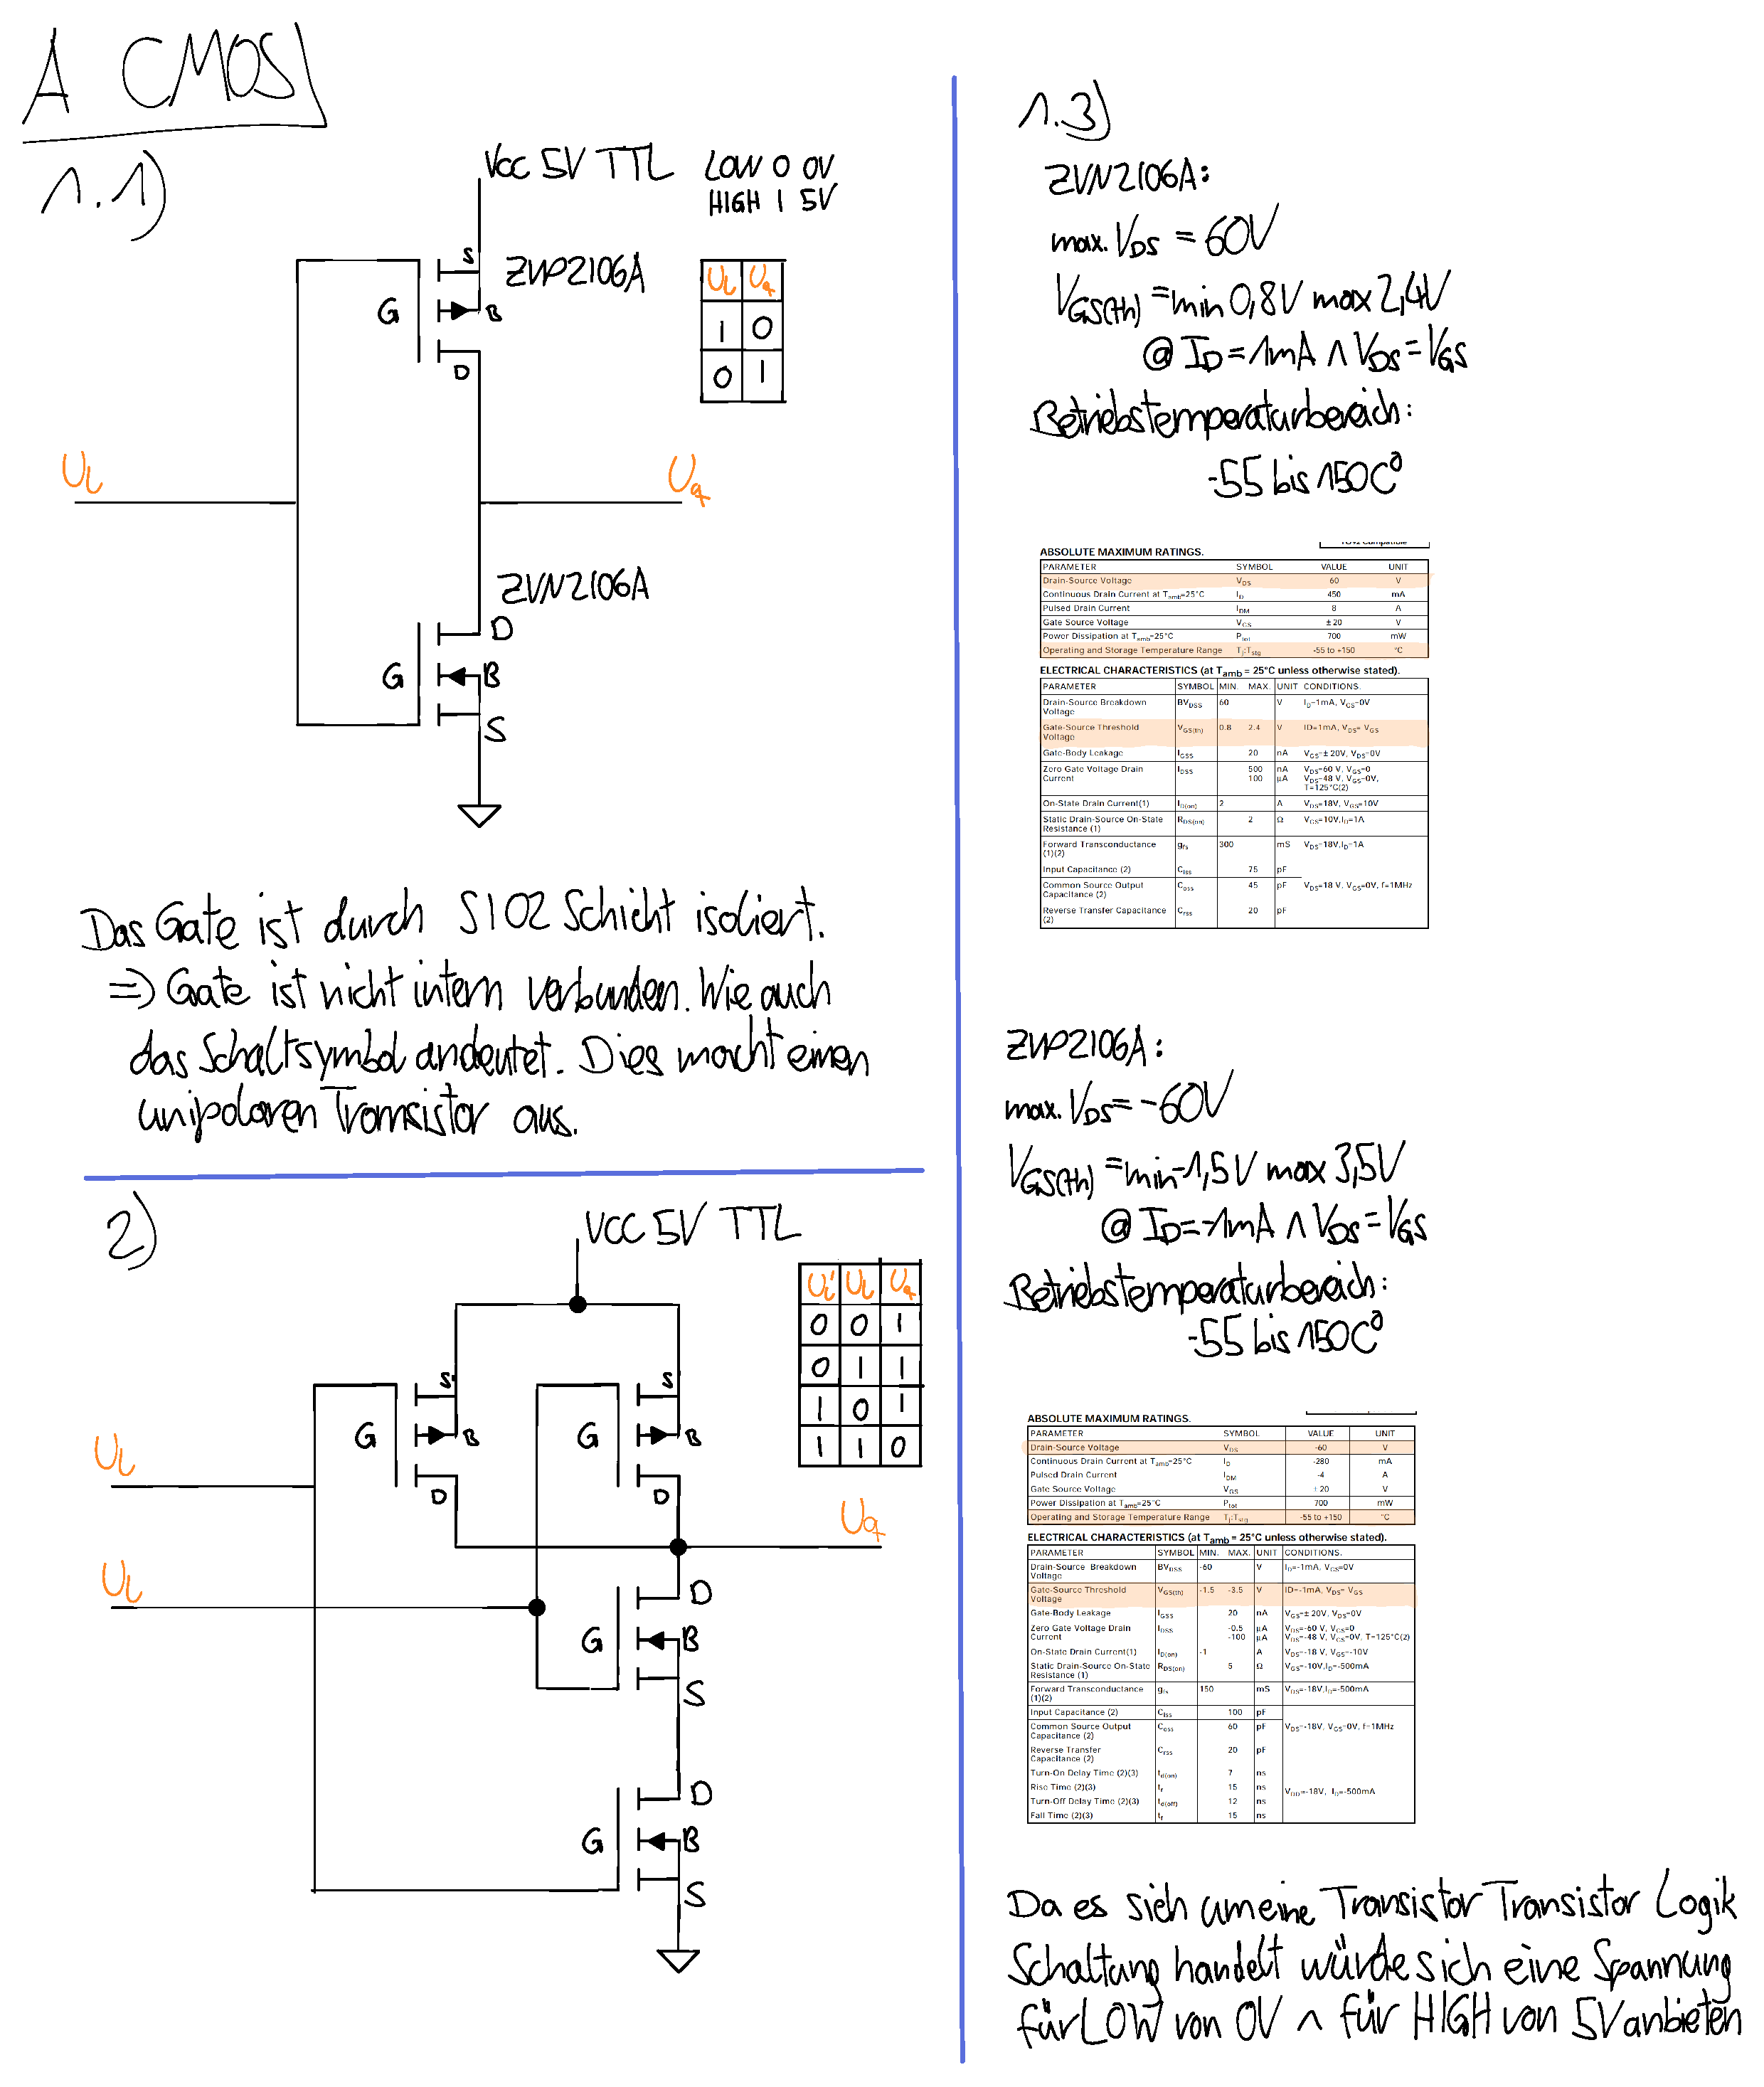
\includepdf[pages=-,
%      addtotoc={
%          1, section, 2, Vorbereitung, sec:Vorbereitung
%      }]{./figures/CMOS-Logik1.pdf}
% \includepdf[pages=-]{./figures/CMOS-Logik2.pdf}
% 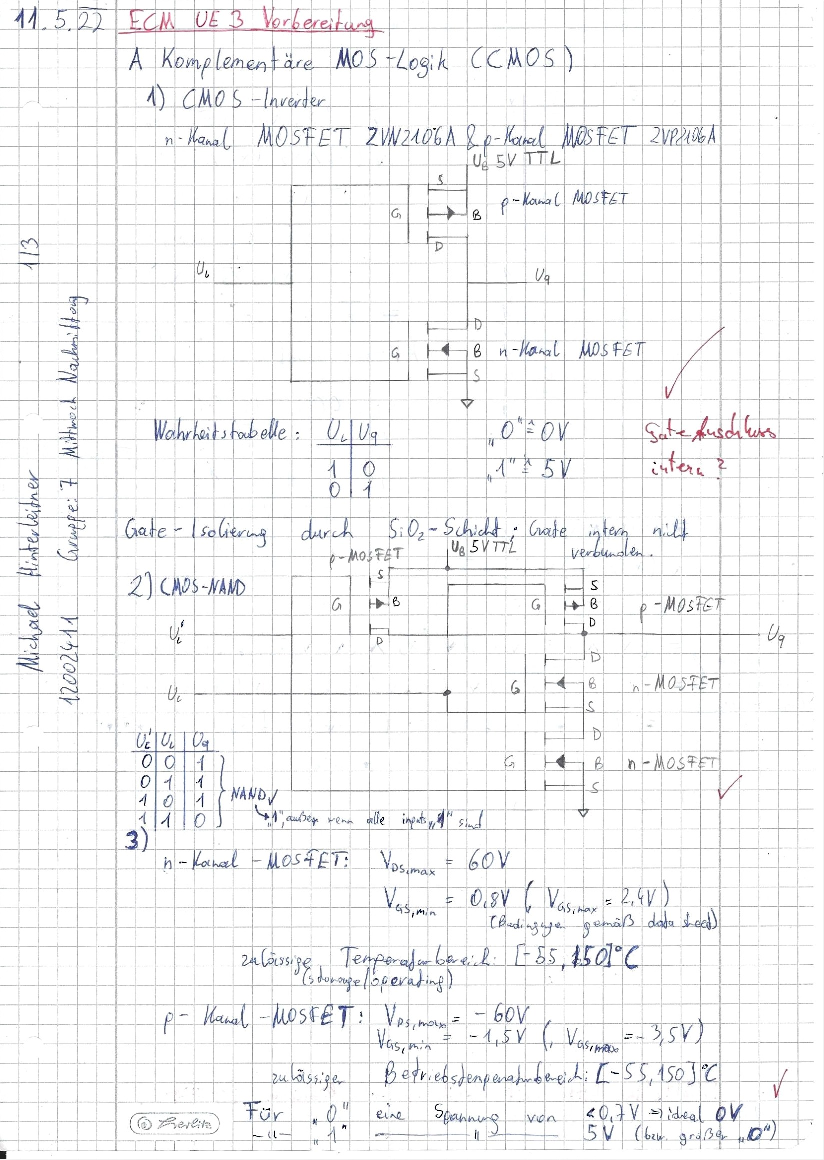
\includepdf[pages=-]{./ecm3_vorbereitung.pdf}


% zu 3: Grundlagen In den Grundlagen sollen die später verwendeten Formeln
% stehen und kurz erklärt werden, dabei ist es nicht notwendig Formeln
% herzuleiten. Quellenangaben sind an dieser Stelle von Vorteil, weil Sie so
% schnell die betreffenden Stellen in Unterlagen finden. In den Rechnungen
% werden grundlegende Annahmen skizziert und begründet und dann mit diesen
% Annahmen, die für die Schaltungen notwendigen Werte berechnet. Dabei kann
% auch gleich auf die später wirklich verwendeten Werte Bezug genommen werden -
% wir verwenden bei den Widerständen zum Beispiel von den Normwert-Reihen die
% E12 und/oder E24 Serie (nach DIN 41426 bzw. IEC 63).
\section{Grundlagen}\label{sec:Grundlagen}
%in Grundlagen
Operationsverstärker (kurz 'OPV oder 'OpAmp') dienen grundlegend der Verstärkung von 
Gleichspannungen. Sie besitzen einen nicht-invertierenden, der meist mit einem 
Plus, und einen invertierenden Eingang, der mit einem Minus dargestellt wird. Zu 
beachten ist, dass die Verstärkung auf die Differenzspannung der beiden Eingänge 
wirkt. Je zwei zusätzliche Anschlüsse finden sich für die positive und negative 
Betriebsspannung und für den Offsetabgleich, damit bei keiner Eingangsspannung 
auch keine Ausgangsspannung auftritt - dieser wird also in einer externen 
Schaltung durchgeführt.

\begin{figure}[H]
    \centering
    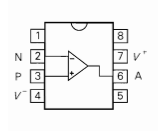
\includegraphics[width=6cm, height=6cm,keepaspectratio]{./figures/pics/pins.PNG}
    \caption{Schematische Darstellung der Pinbelegung eines klassischen Operationsverstärkers. Hierbei bezeichnet 2 den invertierenden, 3 den nicht-invertierenden Eingangskanal, 6 den Ausgang, 4 den Anschluss für die negative sowie 7 den Anschluss für die positive Betriebsspannung, 1 und 5 die Pins für den Offsetabgleich und 8 einen freien Pin.  \cite{tietze}}
    \label{fig:pin_anschl}
\end{figure}

In \autoref{fig:pin_anschl} sind die Pins eines Operationsverstärkers, wie er auch 
in der Laborübung verwendet wurde, zu sehen. Dabei ist zu beachten, dass jeder nicht 
belegte Pin auf Masse gelegt werden soll.

Es gibt vier grundlegende Arten der Verwendung von Operationsverstärkern, darunter
der nicht-invertierende Betrieb, bei dem das Eingangssignal nur auf den nicht-invertierenden 
Kanal gelegt wird und der invertierende auf Masse gelegt wird. Analog funktioniert der invertierende 
Modus, bei dem das Signal anstelle nun an den invertierenden Eingang gelegt wird, wodurch die Ausgangsspannung 
zusätzlich zur Verstärkung noch zum Eingangssignal invertiert wird. Beim Differenzbetrieb werden an 
beide Eingänge Signale angelegt und die Differenzspannung verstärkt. Im Falle des Gleichtaktbetriebs 
liegt das gleiche Eingangssignal an den beiden Eingängen an, wodurch es theoretisch keine Differenzspannung 
und Verstärkung geben sollte - in der Realität resultiert allerdings eine Verstärkung, die als 
Gleichtaktverstärkung bezeichnet wird.

Da der Operationsverstärker ohne zusätzliche Verkopplung sehr stark frequenzabhängig ist und 
nur eine geringe Bandbreite gewünscht verstärkt, wird eine Gegenkopplung vom Ausgang zum Eingang 
durchgeführt, wodurch die Verstärkung zwar abnimmt, die Bandbreite jedoch stark vergrößert wird. 
Die Bandbreite wird wie gewohnt durch die Grenzfrequenz charakterisiert, bei welcher die Verstärkung 
noch \SI{70}{\%} der maximalen beträgt. Wenn nun beispielsweise ein Kondensator in der Rückkopplung verbaut wird, 
handelt es sich um eine Integratorschaltung, die im zweiten Teil der Laborübung untersucht wird.

Die resultierende Verstärkung lässt sich gemäß \autoref{eq:ver} als Verhältnis der Ausgangs- $U_a$ zur Eingangsspannung $U_e$ berechnen.
\begin{equation}
	V=\frac{U_a}{U_e}
	\label{eq:ver}
\end{equation}


% zu 4: Versuchsdurchführung In diesem Punkt wird die Durchführung der
% einzelnen Aufgaben beschrieben. Im Simulationsteil ist die simulierte
% Schaltung mit allen Analyseparametern darzustellen. Im praktischen Teil sind
% die verwendete Geräte sowie die gemessenen Werte der verwendeten Bauteile
% anzugeben. Außerdem sind durchgeführte Funktionsüberprüfungen der Bauteile
% (Dioden, Transistor, etc.) anzuführen. Die Messergebnisse bzw. Oszillogramme
% sind mit Angabe der verwendeten Messgeräte anzugeben. Oszillogramme werden
% vom verwendeten Oszilloskop als Daten auf einen USB-Stick ausgegeben und
% können in das Protokoll aufgenommen werden. Das gleiche gilt für Schaltungen
% bzw. Ergebnissen von Simulationen. Es ist auf eine klare Darstellung der
% Messergebnisse und –auswertung zu achten (Tabellen, geeignete Grafiken). Die
% originalen, während des Versuchs angefertigten Aufzeichnungen sind dem
% Protokoll beizufügen. 
\section{Versuchsdurchführung}\label{sec:versuchsdurchfuehrung}
%Für den praktischen Teil an der Steckplatine wurden Widerstände der E12-Reihe,
%mit denen die in der Vorbereitung angegebenen respektive errechneten Werte
%angenähert wurden, verwendet.
Da die exakten Komponenten für die logischen Gatter nicht in
\textit{LTspice} zur Verfügung standen, wurden funktionstüchtig-äquivalente
Bauteile in der Simulation verwendet. Die Gegenstücke in der Simulation wurden
unten angeführt.
Die verwendeten Geräte sind \autoref{tab:geraeteliste} zu entnehmen.

\begin{table}
  \caption{Tabelle der verwendeten Geräte}
  \label{tab:geraeteliste}
  \centering
  \begin{tabular}{l|l|l}
    \hline
   \multicolumn{3}{ c }{\textbf{Geräteliste}} \\
    \hline
    \textbf{Gerät/Bauelement} & \textbf{Typ} & \textbf{In Simulation}\\
    \hline
    % Oszilloskop & \textit{Tektronix TDS 2002}\cite{oszilloscope}\\
    % Funktionsgenerator & \textit{H-TRONIC FG250D}\cite{funktionsgenerator} \\
    Netzgerät & nicht bestimmbar\\
    %Multimeter & \textit{Fluke 175 TrueRMS}\cite{fluke175} \\
    % todo references
    NOT-Gatter     &  \textit{74LS04}\cite{74LS04} & 74HCT04      \\
    2x-NAND-Gatter &  \textit{74LS00}\cite{74LS02} & 74HCT00       \\
    3x-NAND-Gatter &  \textit{74LS10}\cite{74LS27} & 74HCT10      \\ 
    JK-MS-FF       &  \textit{74LS109}\cite{}      & 74HCT109  \\
    \hline
  \end{tabular}
\end{table}

\paragraph{Entprellter Schalter}\label{sec:schalter_aufbau}
%TODO text erklaeren wie der Schalter angesteuert wird und wo er verwendet wurde
Der entprellter Schalter wird als Signalgeber für die logischen Schaltungen und
Gatter verwendet. Der Aufbau dieses Schalters ist in
\autoref{fig:aufbau_schalter} ersichtlich, jedoch ist noch der \textit{GND} mit
Ground und \textit{VCC} mit \SI{5}{\volt} zu beschalten, damit das Signal von
den Schaltern für die jeweilige Betriebsart abgegriffen
werden kann.

Jeder dieser Schalter hat hierbei eine Standard-\textit{HIGH}- bzw.
\textit{LOW}-Betriebsart.

\begin{figure}[H]
  \centering
    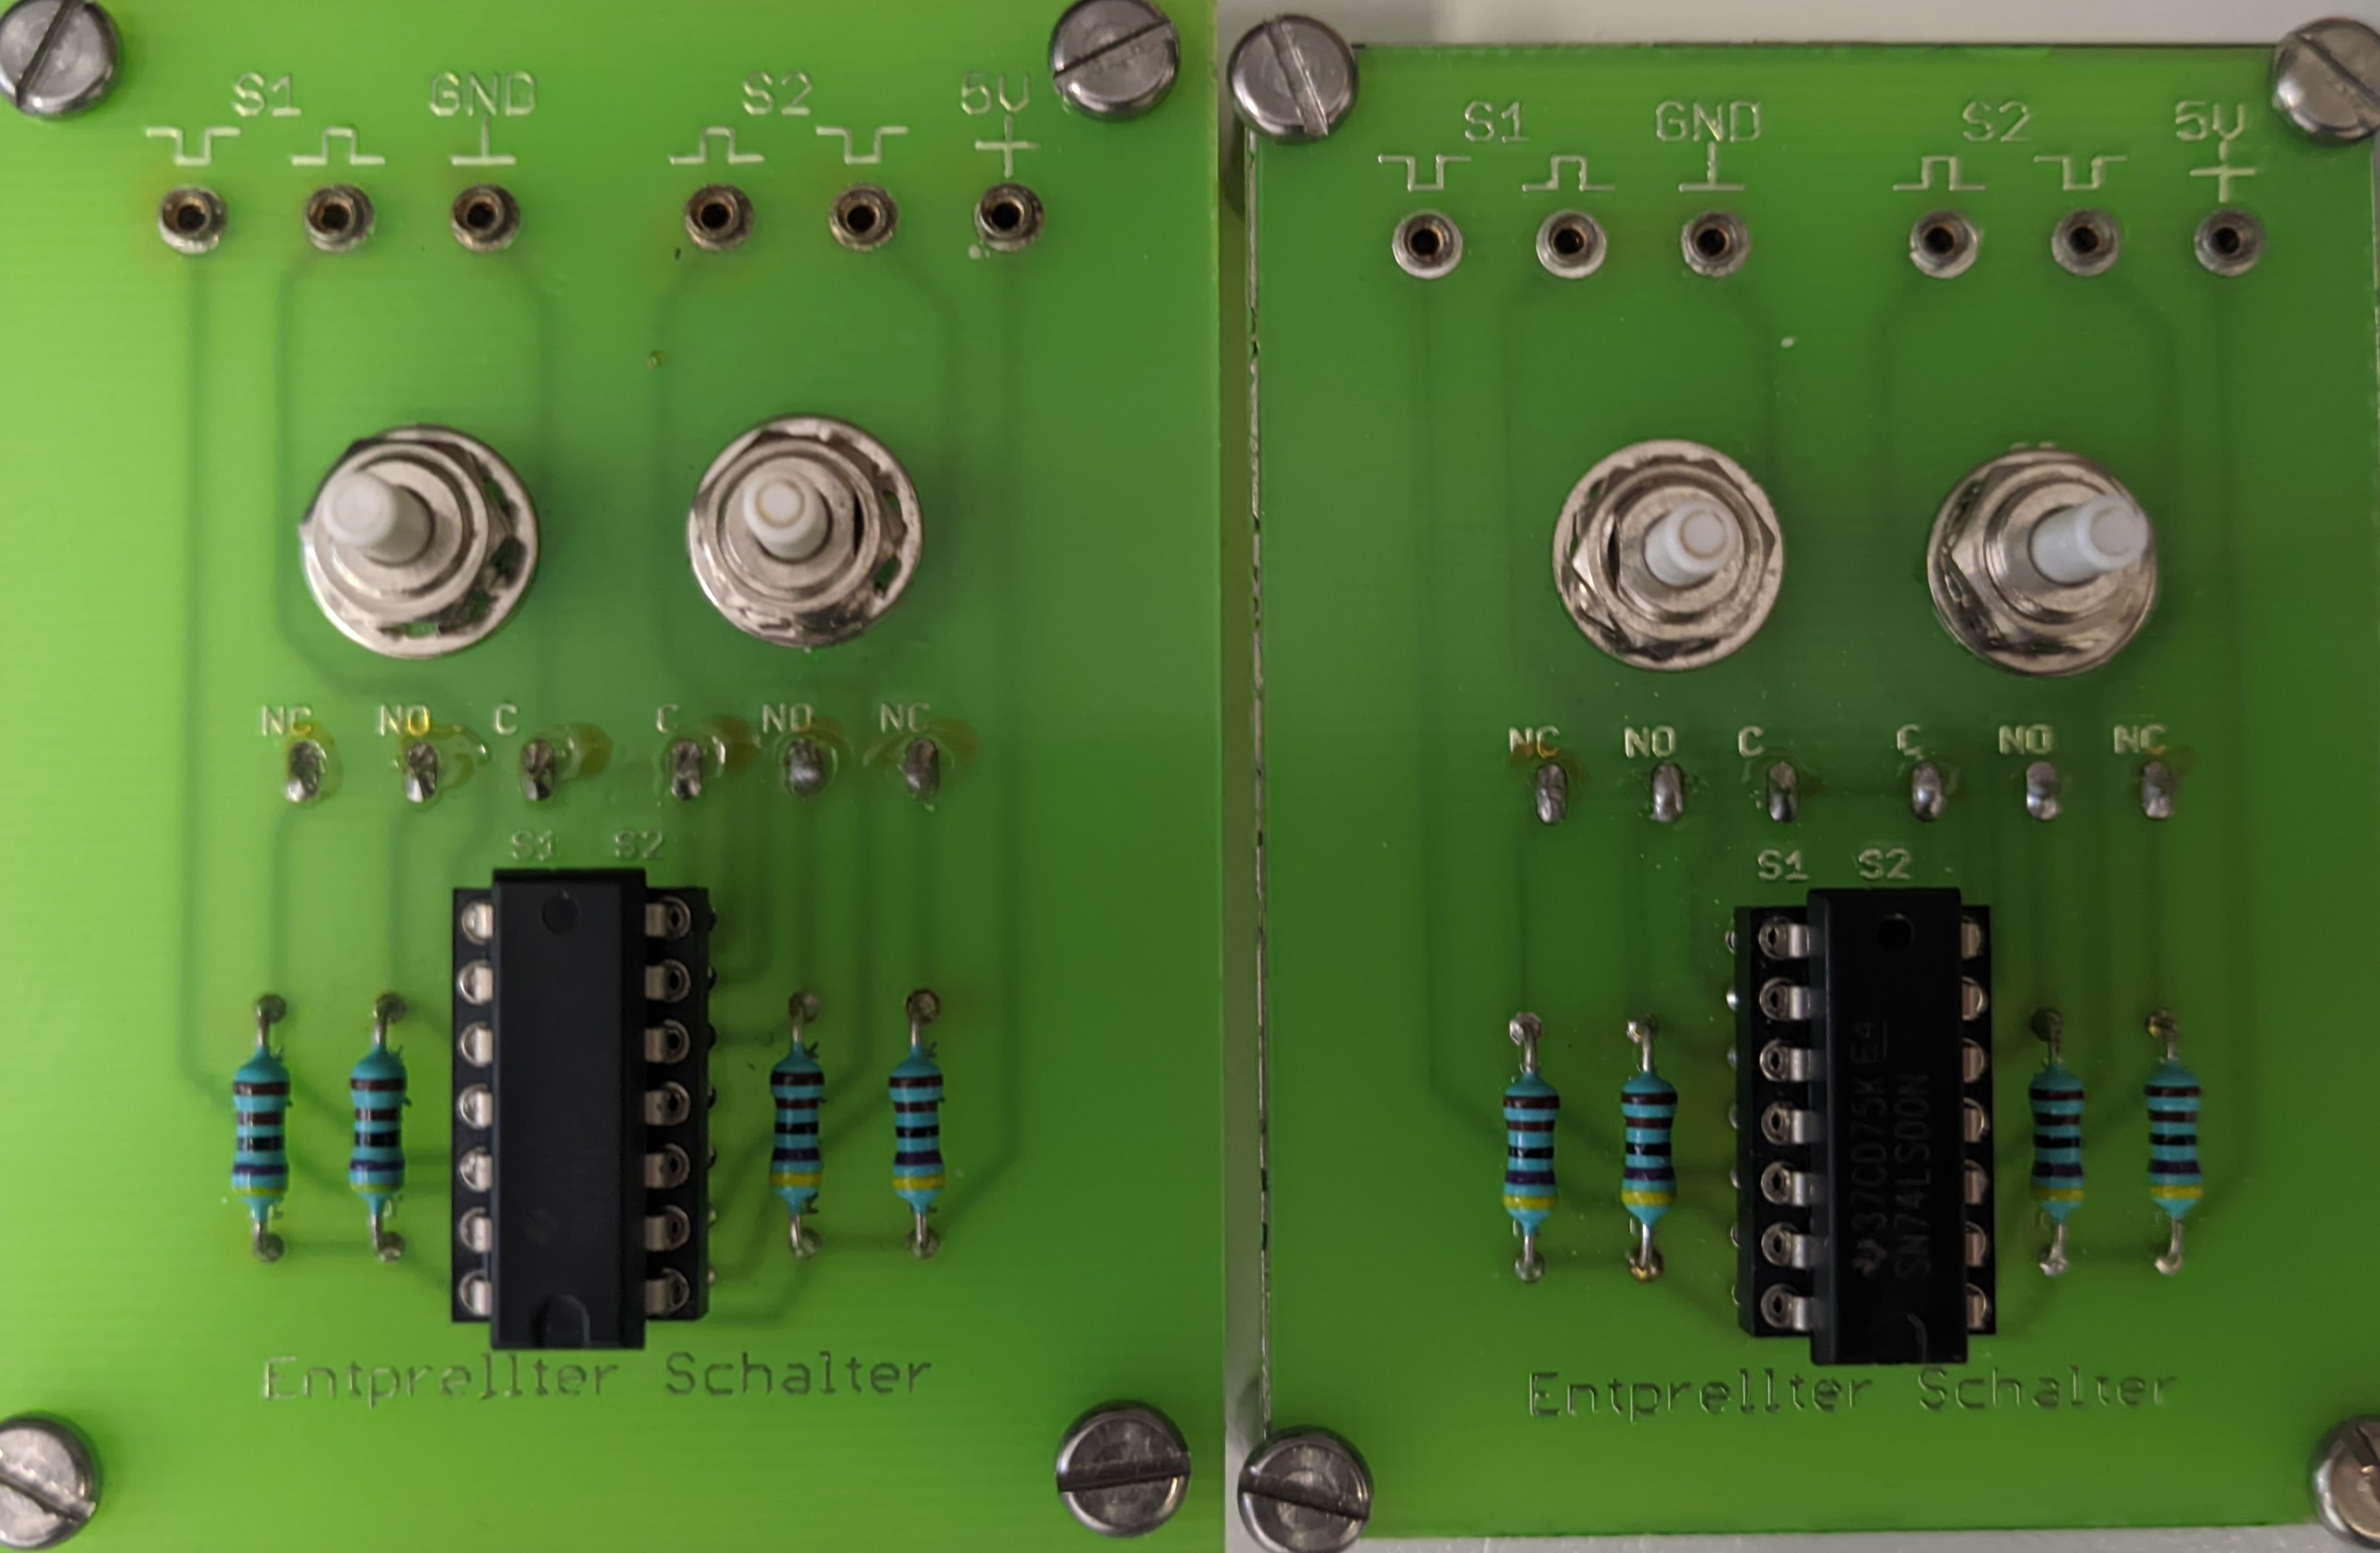
\includegraphics[width=0.95\textwidth]{./figures/messungen/schalter.jpg}
  \caption{Dies sind die zwei entprellten Schalterplatinen mit je zwei Schalter
    ($S1$,$S2$) die entweder mit Standard-\textit{HIGH} oder -\textit{LOW} verwendet
    werden können. Diese werden durch Beschalten des \textit{GND} und der \SI{5}{\volt}
    Betriebsspannung in Betrieb genommen}
  \label{fig:aufbau_schalter}
\end{figure}

% dabei sollte man den schalter auf eingangs und Ausgangsspannungen ueber
% pruefen damit man sieht ob er fuer logische schaltung ueberhaupt brauchbar
% ist

\paragraph{LED Leiste}
%TODO text erklaeren wie der Leiste angesteuert wird und wo er verwendet wurde
Damit die Eingangssignale und Ausgangssignale der logischen Schaltungen
dargestellt werden können, wird eine LED-Leiste verwendet. Diese besteht aus
mehreren LEDs mit Vorwiderständen und ist in \autoref{fig:aufbau_led} dargestellt und
unterstützt bis zu 8 Aus- bzw. Eingangssignale. Die hier verwendete LED-Leiste
hat einen Common-Ground und somit werden positiven Spannungssignale direkt an den
verschiedenen Anschlüssen angelegt um die LED zum Leuchten zu bringen.

\begin{figure}[H]
  \centering
  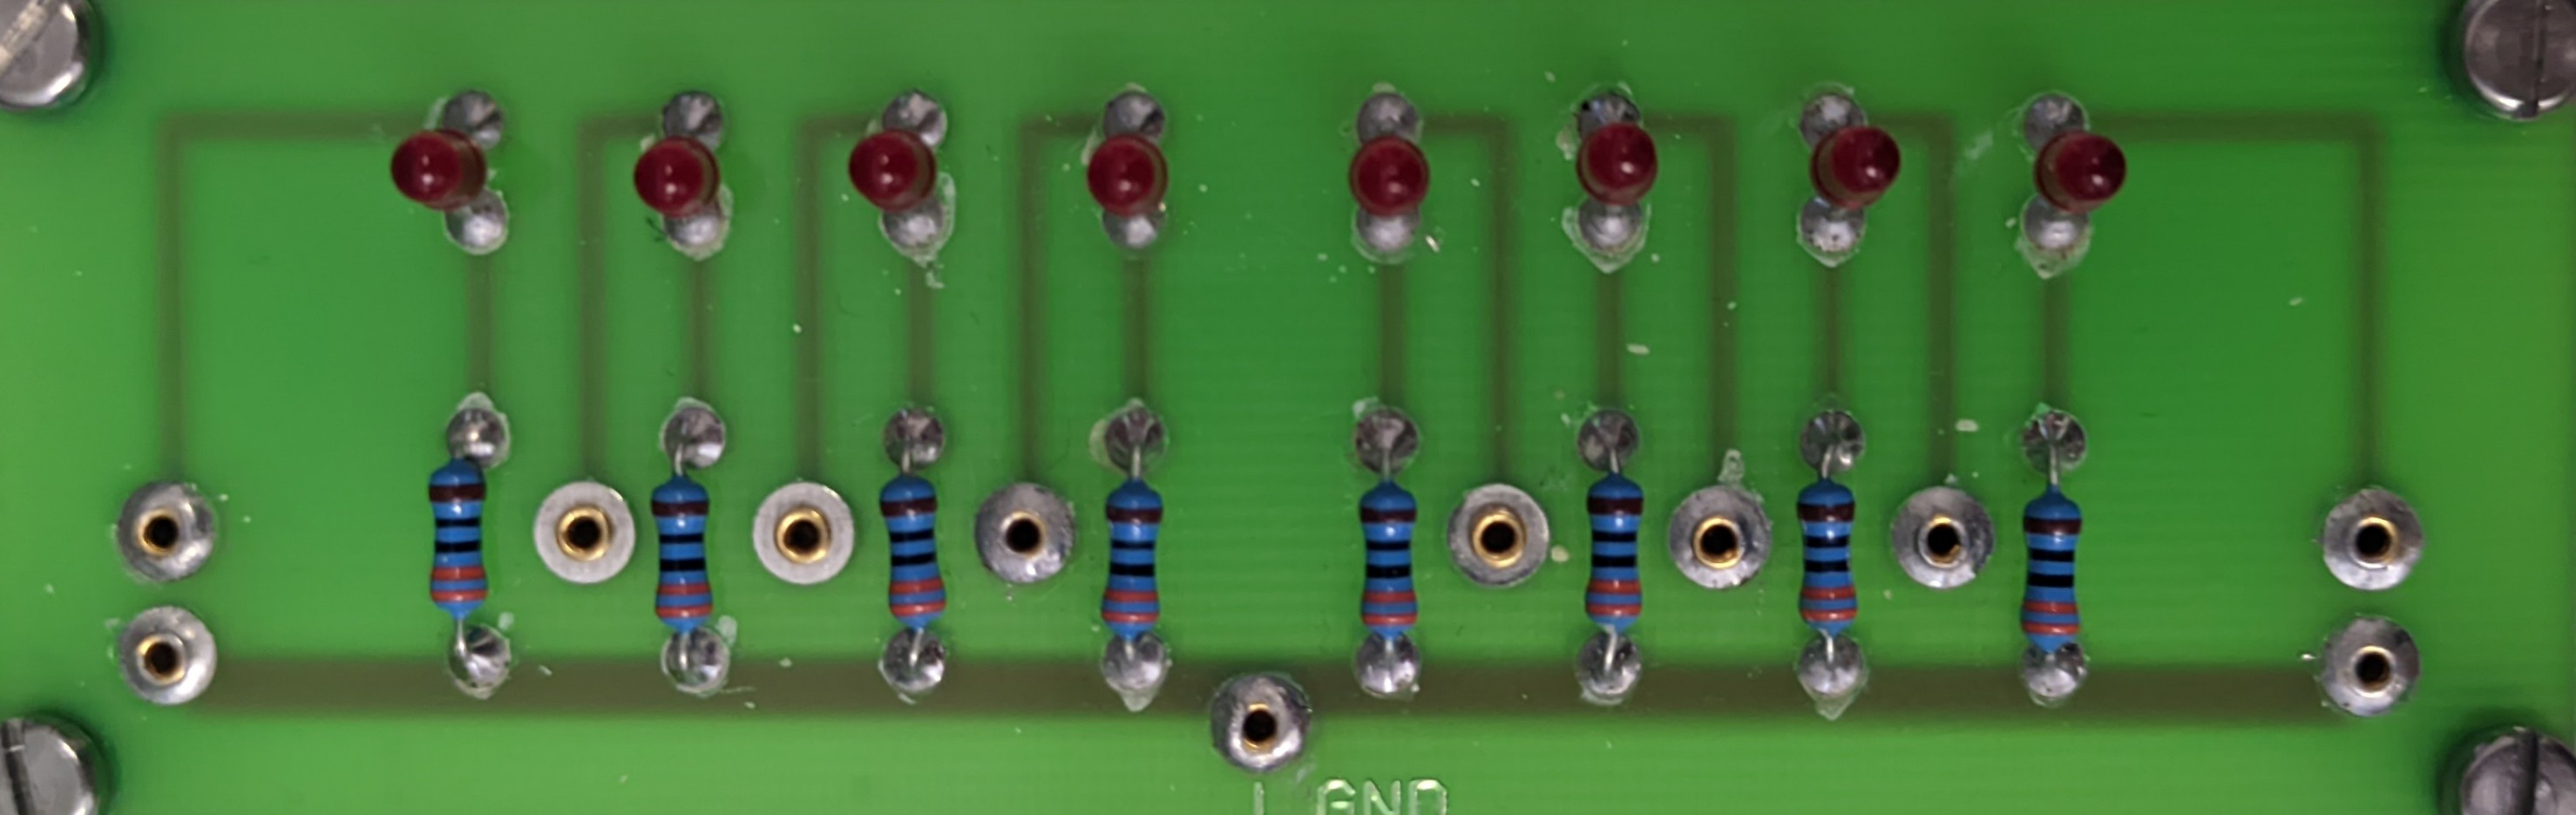
\includegraphics[width=\textwidth, height=6cm,keepaspectratio]{./figures/messungen/ledleiste.jpg}
  \caption{Dies ist die LED-Leiste, welche 8 LEDs mit je einem Vorwiderstand
  hat. Sie ist in Common-Ground-Konfiguration und wird verwendet, um Signal
  anzeigen zu können.}
  \label{fig:aufbau_led}
\end{figure}

Damit die Aufnahmen der Schaltungen übersichtlich bleiben, wurden diese meistens
von den Aufnahmen weggeschnitten und deren Funktion in der jeweiligen Grafik
mittels \textit{LED} dargestellt oder in der Beschriftung gekennzeichnet bzw.
erwähnt.


\subsection{Master-Slave-Flip-Flop}


% 2.1 Die Schaltung ist mit LTspice zu simulieren. Die Eingangspegel sowie die
% Ausgangspegel sind digital darzustellen  
\subsubsection{Simulation}

Die Schaltung des JK-Master-Slave-Flip-Flop (JK-MS-FF) wurde gemäß der
\nameref{sec:Aufgabenstellung} in \autoref{fig:sim_aufbau_jk} in
LTSpice aufgebaut und simuliert. Diese Schaltung wurde mit fünf Eingangspins
und zwei Ausgangspins konstruiert. Die fünf Eingangspins sind \textit{J C K R S},
wobei \textit{S R} die direkten Set und Reset (bzw. PRESET \& CLEAR), \textit{C} das
Clocksignal, \textit{J K} die normalen SET und RESET Pins als Eingänge des
JK-Master-Slave-Flip-Flop sind. 

\begin{figure}[H]
  \centering
  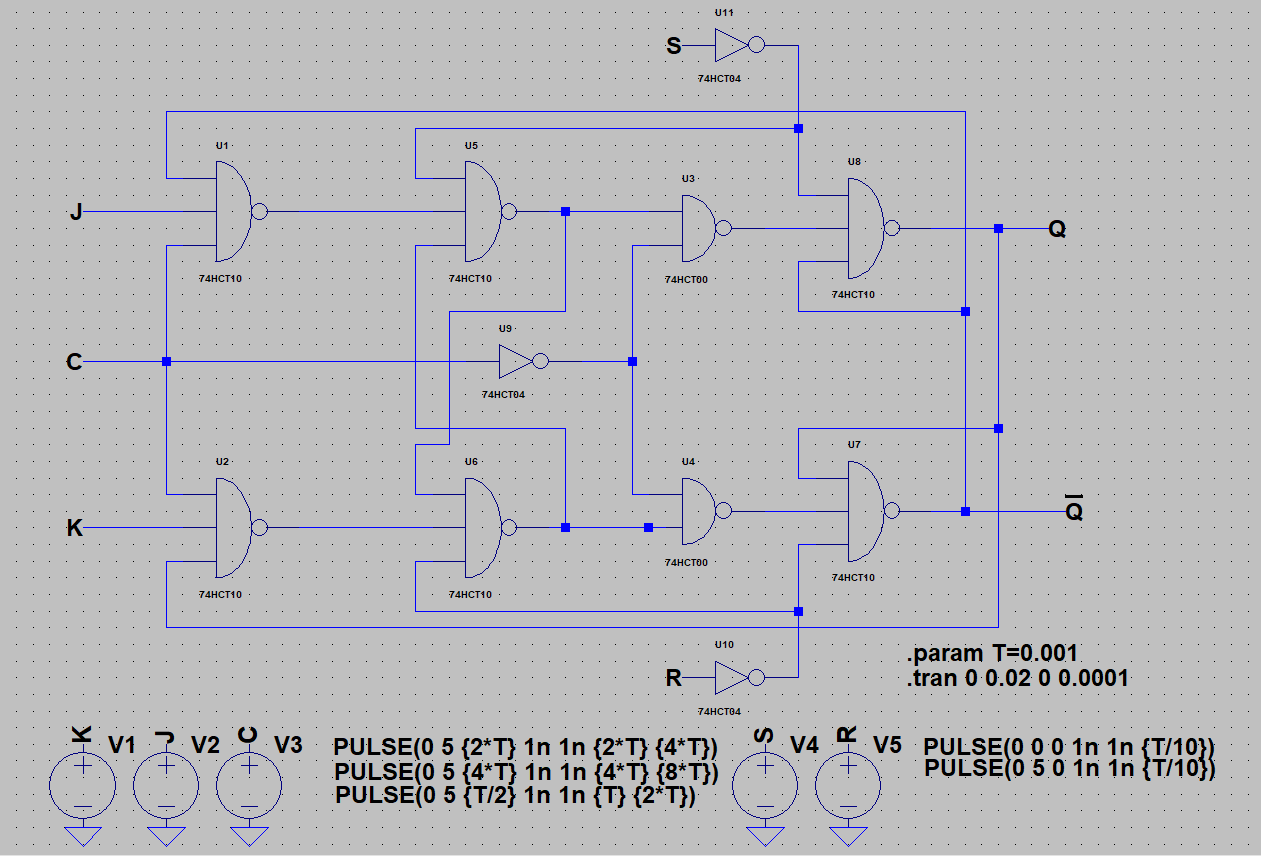
\includegraphics[width=0.95\textwidth]{./figures/sim/jk/aufbaujk.png}
    \caption{Dieser Schaltplan zeigt, den Aufbau eines
      JK-Master-Slave-Flip-Flops. Die verwendeten Bauteile sind in der Grafik
      abgebildet und in \autoref{tab:geraeteliste} nochmals angeführt. Die
      verwendeten Simulationskomponenten im Schaltplan
      ersichtlich.
    Dabei ist:\\
    \textit{J}$\dots$ normaler Set-Eingang\\
    \textit{K}$\dots$ normaler Reset-Eingang\\
    \textit{C}$\dots$ Clocksignal-Eingang\\
    \textit{R}$\dots$ CLEAR-Eingang\\
    \textit{S}$\dots$ PRESET-Eingang\\
    \textit{Q}$\dots$ Ausgang\\
    \textit{$\Bar{Q}$}$\dots$ Invertierter Ausgang\\
  }
  \label{fig:sim_aufbau_jk}
\end{figure}

Nun wurde das Schaltverhalten bei verschiedenen Eingangssignalkombinationen
simuliert. 
Damit die Simulation mit einem bekannten Zustand starten und die
Simulationszeit somit drastisch verringert werden kann, wurde am Anfang ein
direktes Set-Signal am PRESET-Eingang gegeben.
Um die möglichen Kombinationen der Eingangssignale zu erhalten, wurden
die drei für das Verhalten eines JK-MS-FF wichtigen Eingänge \textit{C K J}
mit PWM-Spannungsquellen beschaltet. Wobei \textit{K} die halbe Frequenz von \textit{C} und \textit{J} die
Halbe von \textit{K} hat. Zudem wurde das Clocksignal in \textit{C} um ein Viertel der
Periodendauer verzögert, damit nie das Schalten der Zustande unklar zu ablesen
ist.
Die Schaltsignale wurden mit PWM-Signal von \textit{HIGH} \SI{5}{\volt} und
\textit{LOW} \SI{0}{\volt} gegeben. Die genauen SPICE-Directives können dem
Schaltplan aus \autoref{fig:sim_aufbau_jk} entnommen werden. Daraufhin wurde
eine zeitliche Transienten-Analyse der Eingangs- und Ausgangsspannungen
durchgeführt, woraus sich \autoref{fig:sim_jk_wahrheit} ergab. Für die
Transienten-Analyse wurde folgende SPICE-Directive \texttt{.tran 0 0.02 0 0.0001}
verwendet.
\begin{figure}[H]
  \centering
  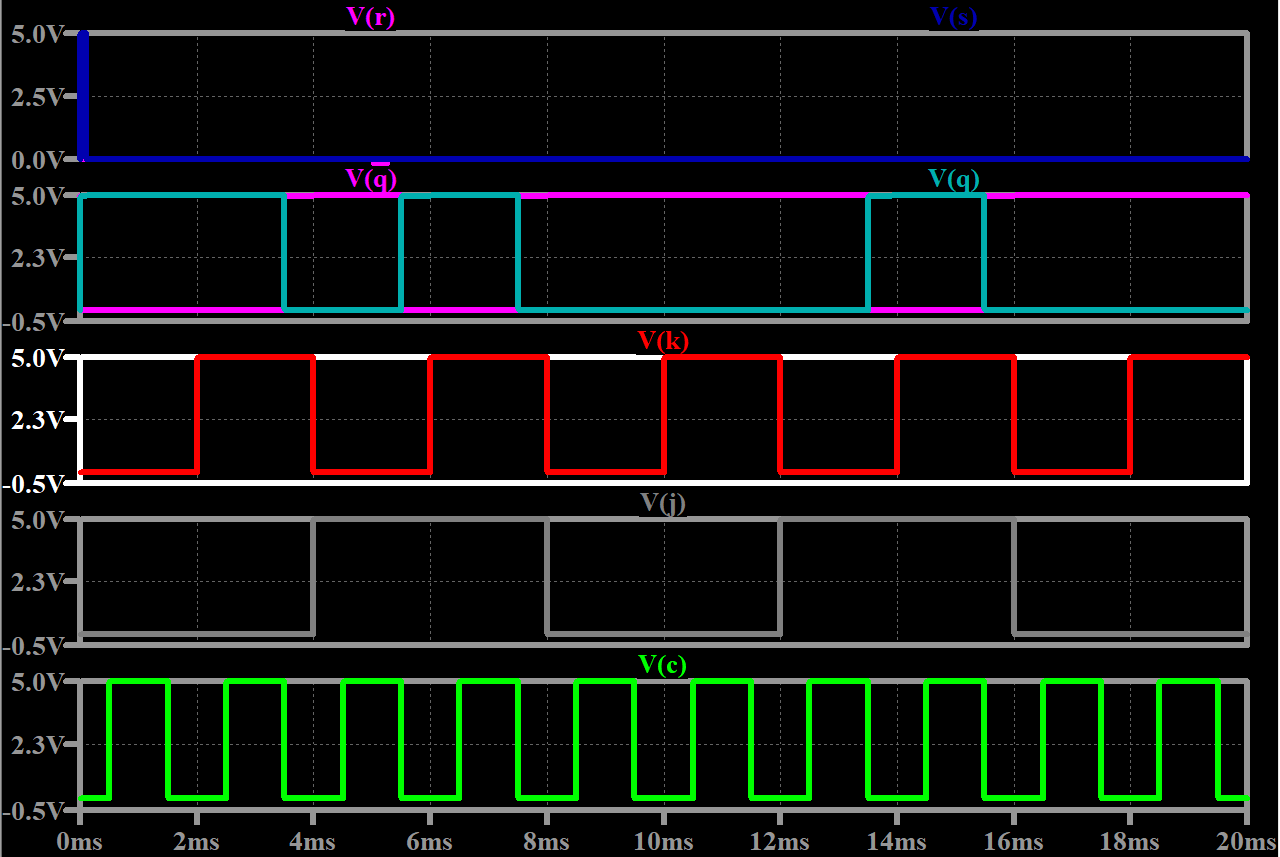
\includegraphics[width=\linewidth, height=7cm]{./figures/sim/jk/WahrheitstabelleJK.png}
  \caption{Diese Grafik spiegelt das simulierte Verhalten des JK-Master-Slave-Flip-Flops (aus
    \autoref{fig:sim_aufbau_jk}) wider, indem alle möglichen Eingangssignale
    durchgeschaltet worden sind und die Response am Ausgang aufgezeichnet
    wurde (entsprechend der Wahrheitstafel). 
    Dabei ist:\\
    \textit{J}$\dots$ normale Set Eingang\\
    \textit{K}$\dots$ normale Reset Eingang\\
    \textit{C}$\dots$ Clocksignal Eingang\\
    \textit{R}$\dots$ CLEAR Eingang\\
    \textit{S}$\dots$ PRESET Eingang\\
    \textit{Q}$\dots$ Ausgang\\
    \textit{$\Bar{Q}$}$\dots$ Invertierte Ausgang\\
    Die SPICE-Directives der Simulation sind in \autoref{fig:sim_aufbau_jk}
    ersichtlich.}
  \label{fig:sim_jk_wahrheit}
\end{figure}

% 2.2 Das JK-Flipflop ist auf dem Steckboard aufzubauen und auf seine
% Funktionalität zu prüfen. Als Pegelgeber werden für das Steckboard vorhandene
% elektronisch entprellte Schalter verwendet. Die Ein- und Ausgangszustände sind
% durch LED´s anzuzeigen und die Funktionalität der Schaltung ist anhand
% ebendieser zu zeigen.  
% 2.3 Die Ergebnisse sind zu dokumentieren und zu diskutieren. 
\subsubsection{Steckboard}
\paragraph{Aufbau des JK-Master-Slave-Flip-Flop}\label{sec:mess_cmos}
% INSPIRATION
%TODO text
Zunächst wird der CMOS-Inverter mittels zweier MOSFETs (einem p-MOSFET \cite{ZVP2106A} und
einem n-MOSFET \cite{ZVN2106A}) wie nach dem Schaltbild (\autoref{fig:sim_aufbau_jk})
aufgebaut. Zur Visualisierung des Eingangszustands $U_l$ und des
Ausgangszustands $U_q$ wurden die LEDs der LED-Leiste parallel dazu geschaltet. Das
Eingangssignal wurde durch einen entprellten Schalter, im Standardzustand
\textit{LOW}, gegeben. Der Aufbau wird in \autoref{sec:schalter_aufbau} dargestellt. Als
Spannungsquelle wurde ein Netzgerät verwendet und auf \SI{5}{\volt}
eingestellt. 

%TODO figure
\begin{figure}[H]
  \centering
    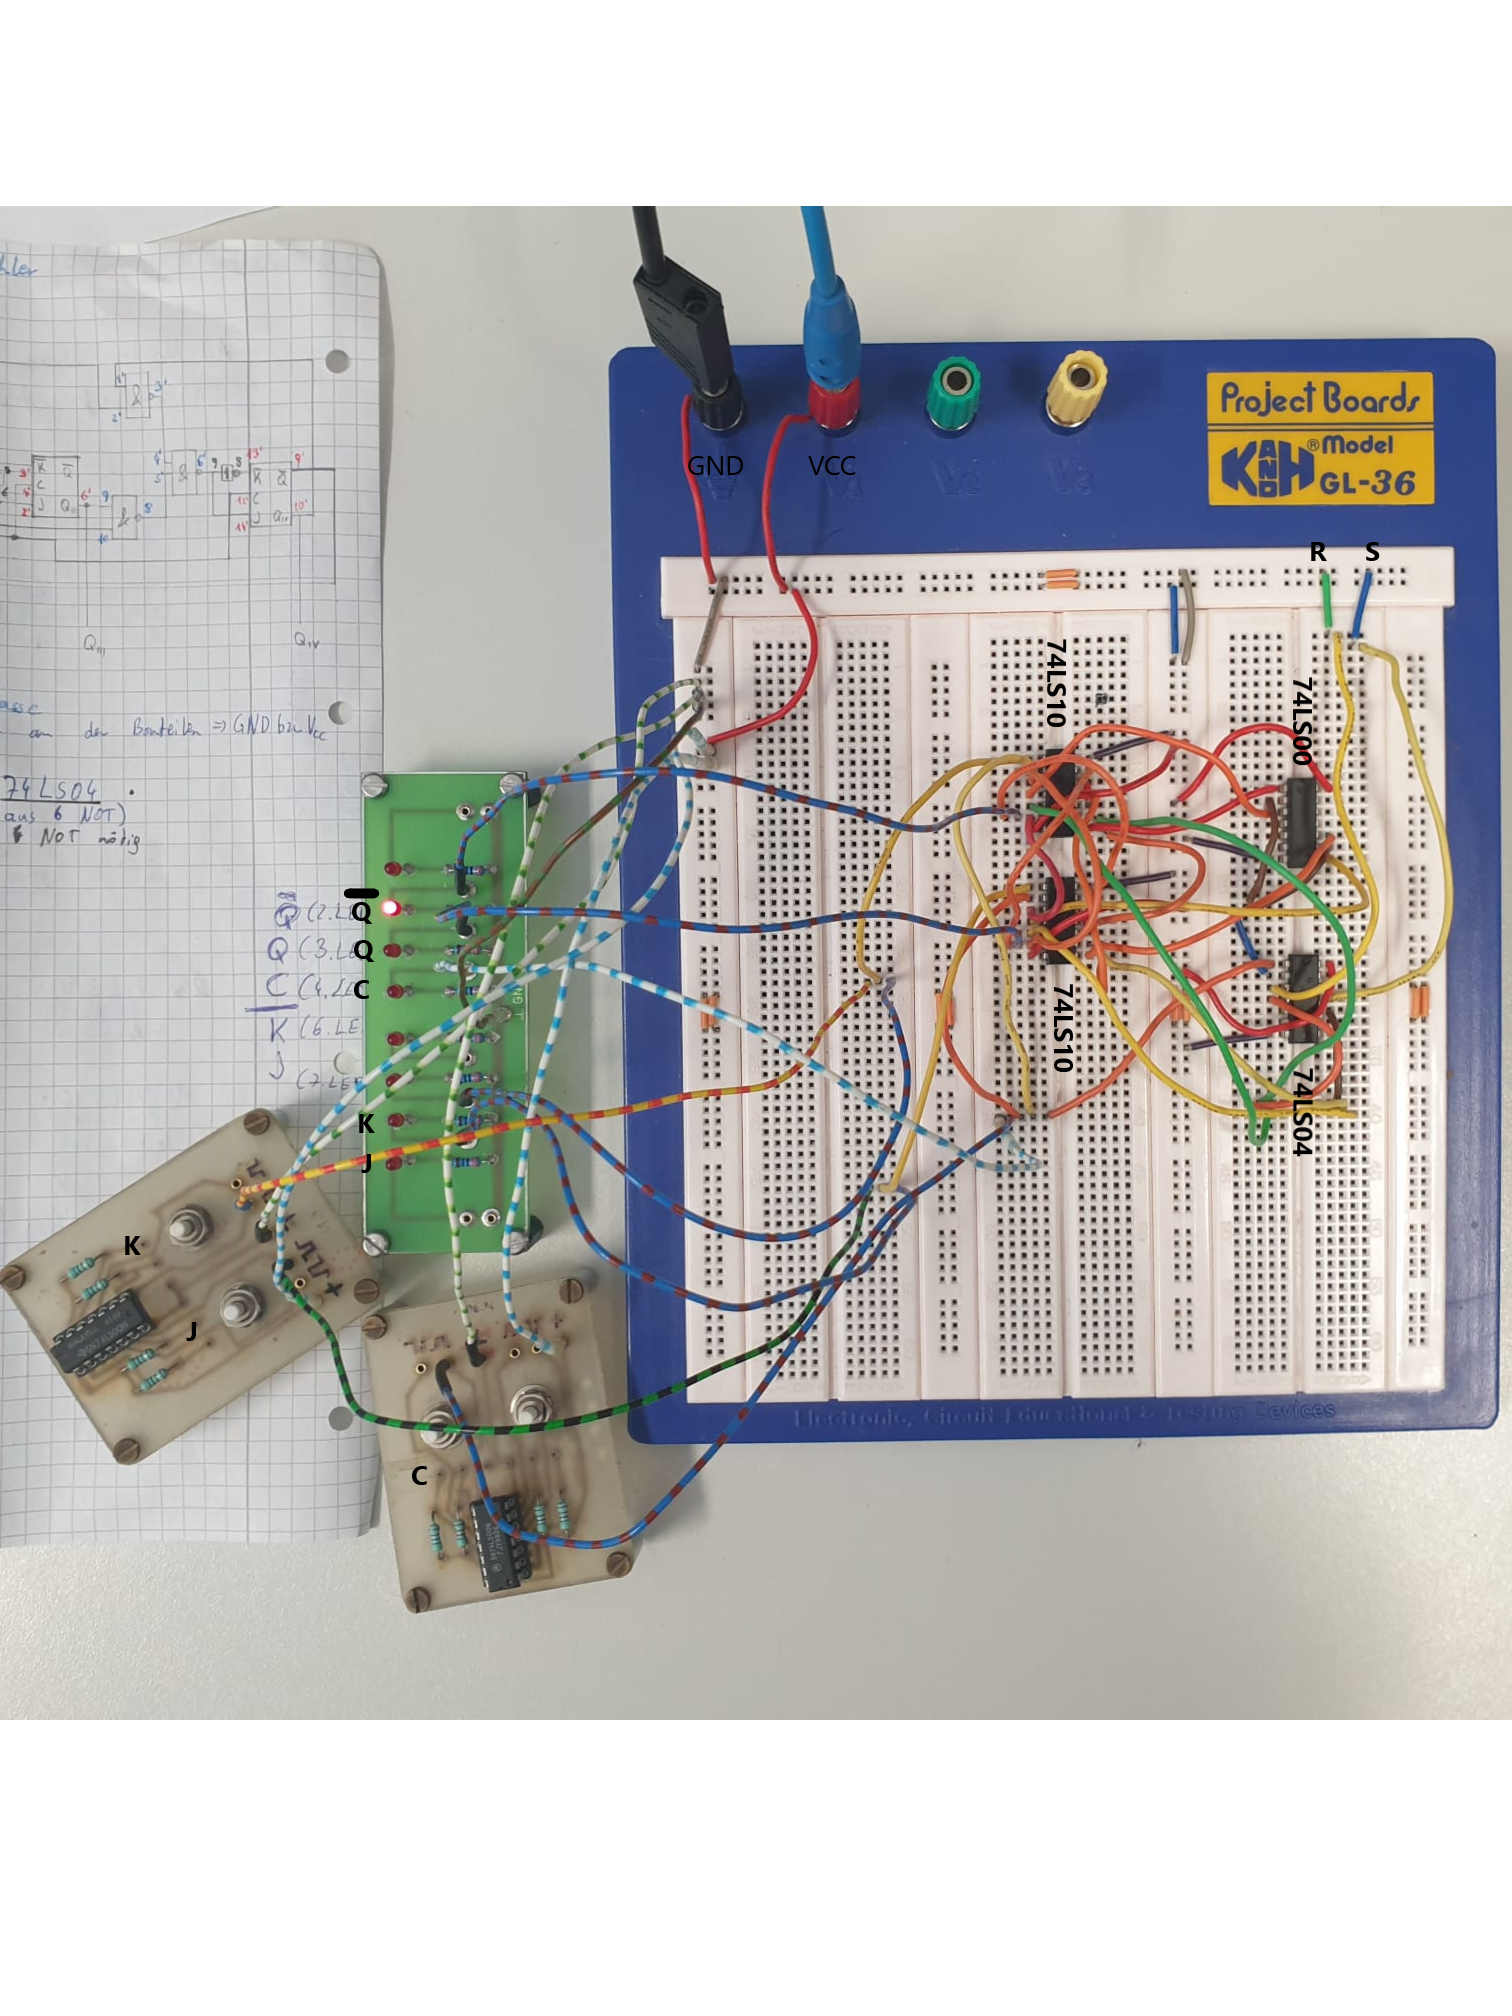
\includegraphics[width=0.95\textwidth]{./figures/messungen/jk/aufbau.png}
  \caption{Dies ist der Aufbau eines JK-Master-Slave-Flip-Flops nach dem
  Schaltplan aus \autoref{fig:sim_aufbau_jk}, wobei:\\
    \textit{J}$\dots$ normale Set Eingang\\
    \textit{K}$\dots$ normale Reset Eingang\\
    \textit{C}$\dots$ Clocksignal Eingang\\
    \textit{R}$\dots$ CLEAR Eingang\\
    \textit{S}$\dots$ PRESET Eingang\\
    \textit{Q}$\dots$ Ausgang\\
    \textit{$\Bar{Q}$}$\dots$ Invertierte Ausgang\\
ist . Der Zustand
  beider kann anhand einer LED in der LED-Leiste abgelesen werden.}
  \label{fig:mess_aufbau_jk}
\end{figure}


Um die Funktionstüchtigkeit des JK-MS-FF's zu überprüfen, wurde die
Wahrheitstafel alle möglichen Schaltsignale der \textit{J K} Eingänge
durchgeschaltet. Die Resultate sind in \autoref{fig:mess_wahrheitstabelle_jk}
ersichtlich.
%TODO text messung
% Als  Pegelgeber wird  für  das  Steckboard  ein vorhandener  elektronisch
% entprellte  Schalter  (mit  Hilfe  eines RS-Flip-Flops)  verwendet.  Der
% Ein-  und Ausgangszustand  ist  jeweils durch  LEDs  anzuzeigen.  Die
% Funktionalität  der Schaltung ist anhand der LEDs zu zeigen.
%TODO figure messung

\begin{figure}[H]
  \centering
    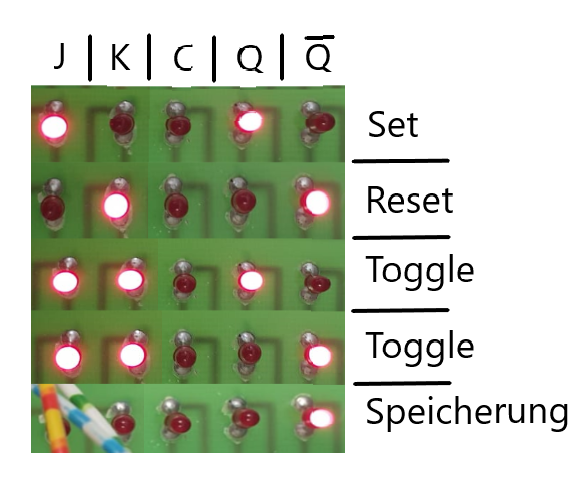
\includegraphics[width=0.95\textwidth]{./figures/messungen/jk/wahrheit.png}
  \caption{Diese Abbildung beinhaltet die gemessenen Eingangs- und
  Ausgangssignale des gebauten JK-Master-Slave-Flip-Flops. Eine leuchtende
  LED entspricht einem \textit{HIGH} Signal, eine nicht leuchtende entspricht
  \textit{LOW}. Zudem ist:\\ 
    \textit{J}$\dots$ normale Set Eingang\\
    \textit{K}$\dots$ normale Reset Eingang\\
    \textit{C}$\dots$ Clocksignal Eingang\\
    \textit{R}$\dots$ CLEAR Eingang\\
    \textit{S}$\dots$ PRESET Eingang\\
    \textit{Q}$\dots$ Ausgang\\
  \textit{$\Bar{Q}$}$\dots$ Invertierte Ausgang}
\label{fig:mess_wahrheitstabelle_jk}
\end{figure}


% INSPIRATION
% \paragraph{Aufbau des CMOS-NAND-Gatters}
% Nun ist die CMOS-NOT Schaltung um zwei weitere MOSFETs erweitert worden, um ein
% NAND-Gatter zu bauen. Dies wurde wie in \autoref{fig:sim_aufbau_nand} aufgebaut.
% Es wurden, wie auch in \nameref{sec:mess_cmos}, entprellte Schalter als
% Pegelgeber und die LED-Leiste zur Visualisierung der Pegel (Signale) verwendet.
% Diese wurden ebenfalls an den geeigneten Abnahme-Stellen angeschlossen; wie diese genau
% angeschlossen wurden ist, der \autoref{fig:mess_aufbau_nand} entnehmbar.




\subsection{Dekadischer synchron 4Bit-Zähler}
% 2.1 Die Schaltung ist mit LTspice zu simulieren. Die Eingangspegel sowie die
% Ausgangspegel sind darzustellen. 
\subsubsection{Simulation}

Das Schaltnetz des Dekadischen synchronen 4Bit-Zähler wurde in
\autoref{fig:sim_aufbau_4bit} aufgebaut. Dabei \textit{CLK} das Eingangssignal
und $Q1$ bis $Q4$ die Ausgänge des Zählers sind wobei $QN$ dem $(N-1)$ten Bit
entspricht. Somit ist wenn nur $Q3$ \textit{HIGH} ist entspricht es der Zahl 4.

\begin{figure}[H]
  \centering
    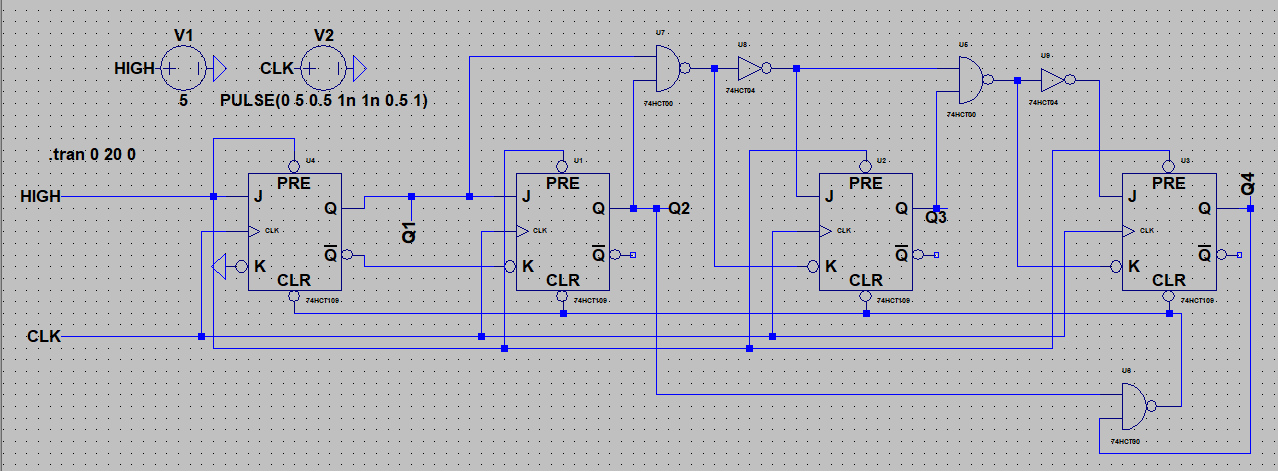
\includegraphics[width=\linewidth]{./figures/sim/4bit/aufbau4bit.png}
    \caption{Dieser Schaltplan beschreibt einen 4Bit dekadischen synchron
      Zähler, wie er in \nameref{sec:Aufgabenstellung} geforderten wurde. Wobei
      \textit{CLK} das zuzählende Eingangssignal ist und $QN$ die $(N-1)$ten
      Ausgangsbits des Zählers sind. Die verwendeten Komponenten können der
      \autoref{tab:geraeteliste} entnommen werden.}
  \label{fig:sim_aufbau_4bit}
\end{figure}

Damit das Zählverhalten des 4Bit dekadischen Zählers untersucht werden kann,
wird das Eingangssignal \textit{CLK} und die Ausgangssignale $Q1$ bis $Q4$
aufgenommen. Das Simulation wurde so lange betrieben, dass ein Overflow
stattfindet und somit der dekadischen Zähler geresetet wird. 

\begin{figure}[H]
  \centering
    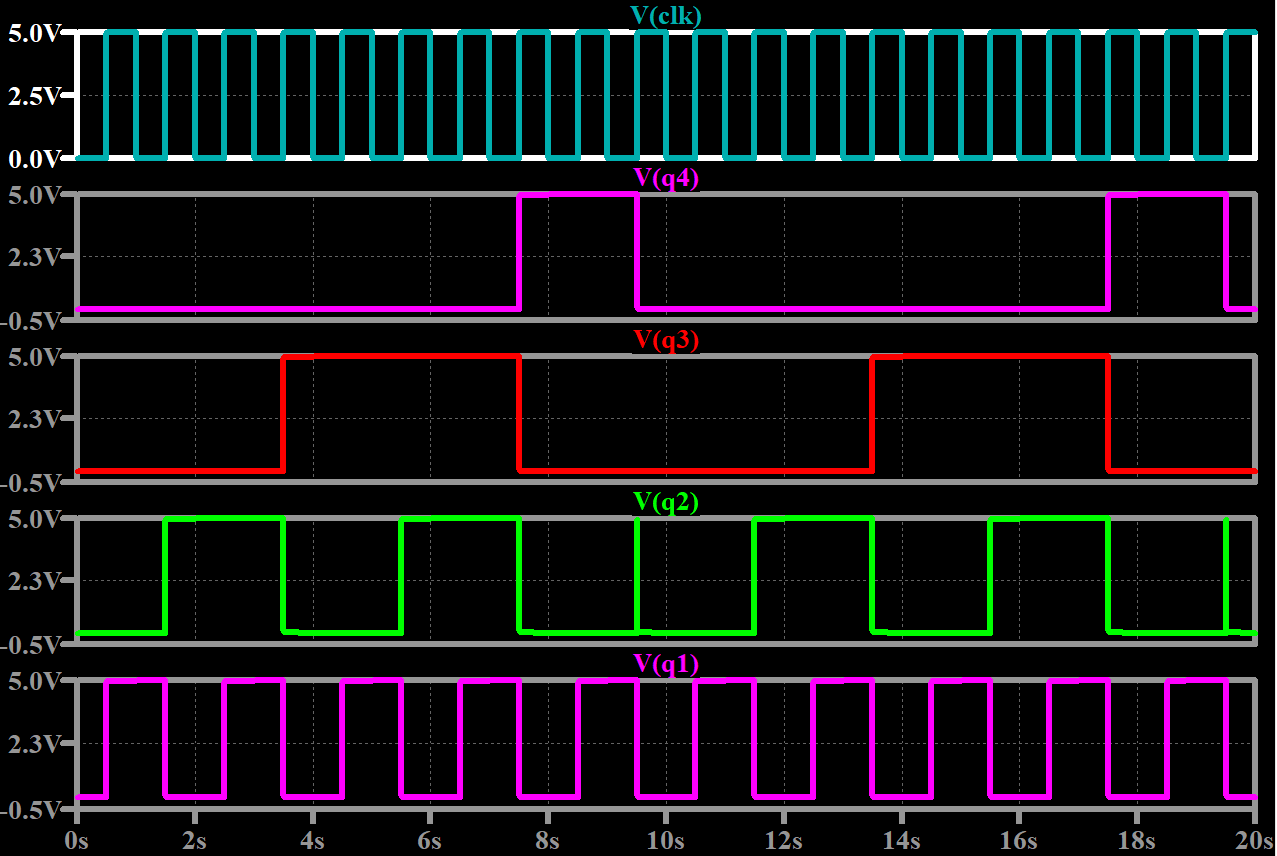
\includegraphics[width=0.95\textwidth]{./figures/sim/4bit/4bitdekawahrheit.png}
  \caption{Diese Grafik spiegelt das Verhalten des
    4Bit dekadischen synchron Zählers (aus \autoref{fig:sim_aufbau_4bit})
    wider, indem bis ein Overflow simuliert wurde und das Eingangssignal und
    alle Ausgangssignale aufgezeichnet wurde (entsprechend Wahrheitstafel).
    Dabei sind $QN$ die $(N-1)$ten Bits des Zählers und \textit{CLK} das zuzählende
    Eingangssignal. Die SPICE-Directive der Simulation ist \texttt{.tran 0 20 0}; die
    Einstellung des Eingangssignals kann der \autoref{fig:sim_aufbau_4bit}
    entnommen werden}
  \label{fig:sim_alarm_wahrheit}
\end{figure}


% 2.2 Die Schaltung ist am Steckboard aufzubauen und ihre Funktionalität zu
% zeigen (siehe Aufgabenstellung A). 
% 2.3 Die Ergebnisse sind zu dokumentieren und zu diskutieren. 
\subsubsection{Steckboard}
Wie in \nameref{sec:Aufgabenstellung} gefordert, galt es eine Schaltung
zu entwickeln, welche durch Anschlagen mindestens zweier Sensoren einen Alarm auslösen
sollte. Diese Schaltung wurde, um die Fehlerquellen zu reduzieren, jedoch aus der
Musterlösung entnommen und nicht die selbst Entworfene verwendet. Die vier
Eingangsgrößen ($x1$, $x2$, $x3$, $x4$) wurden durch vier entprellte
Schalter realisiert. Dabei sind $x1$ \& $x3$ im Standard \textit{LOW} und
$x2$ \& $x4$ Standard \textit{HIGH} Betrieb geschaltet worden, damit die
Alarmanlage bei Signalunterbrechung $x2$ \& $x4$ und einem Signal bei $x1$
\& $x3$ anschlägt. Der Aufbau der Schaltung kann \nameref{fig:mess_aufbau_4bit}
entnommen werden.

%TODO figure
\begin{figure}[H]
  \centering
    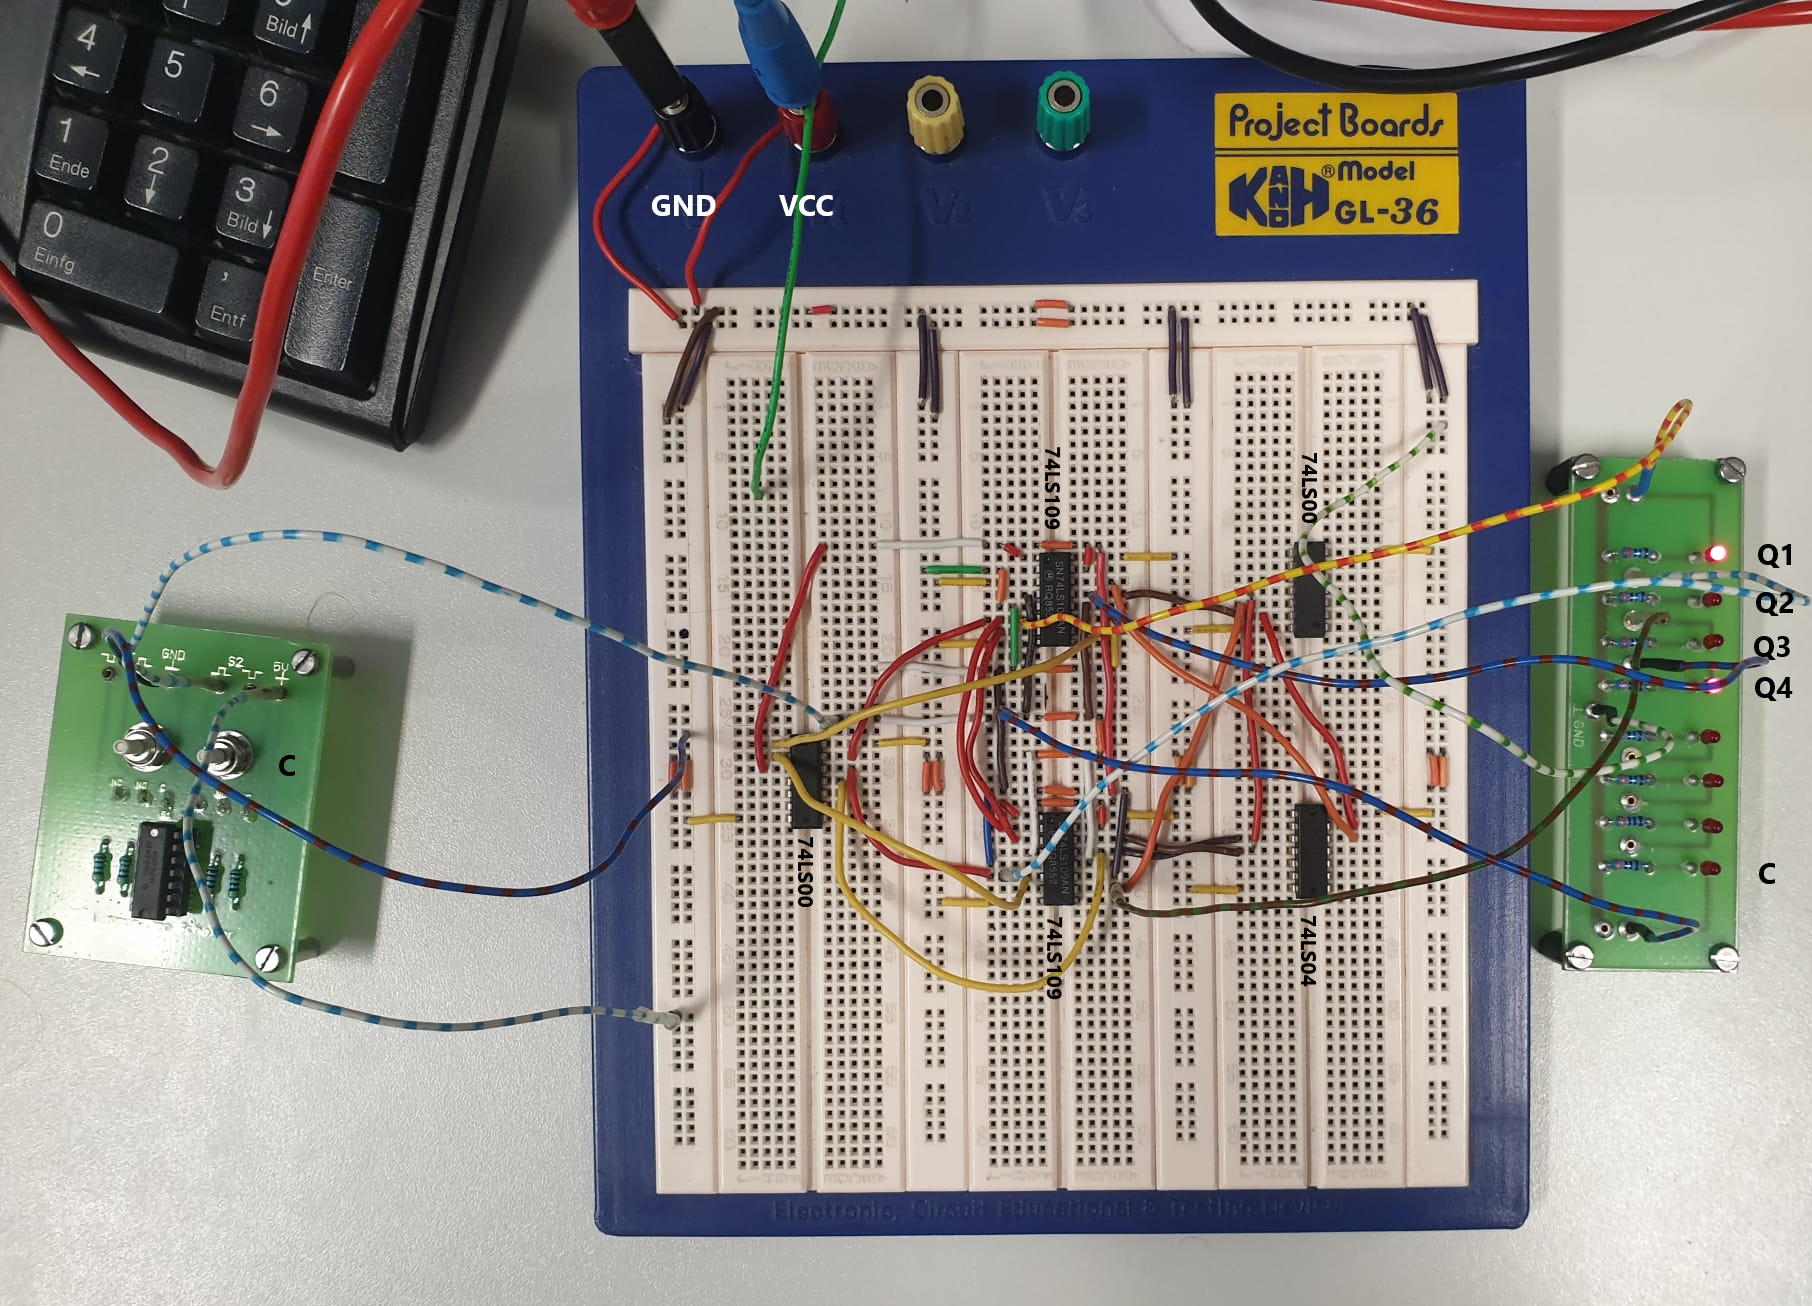
\includegraphics[width=0.95\textwidth]{./figures/messungen/4bit/aufbau.png}
  \caption{Dies ist der Aufbau des dekadischen synchron 4Bit-Zähler nach dem
  Schaltplan aus \autoref{fig:sim_aufbau_4bit}.
Dabei sind $QN$ die $(N-1)$ten Bits des Zählers und \textit{C} das zuzählende
Eingangssignal.
  Die verwendeten Komponenten
  sind der \autoref{tab:geraeteliste} zu entnehmen.}
  \label{fig:mess_aufbau_4bit}
\end{figure}

% Die Ein- und Ausgangszustände sind durch LED´s anzuzeigen und die
% Funktionalität der Schaltung ist anhand ebendieser zu zeigen.
Um die Funktionstüchtigkeit des 4Bit dekadischen synchron Zählers zu
überprüfen, wurde so viele Signale bei \textit{CLK} damit der Zähler bis 10
zählt und dann sich resetet. Somit konnte die Zählfähigkeit der Schaltung
mittels LEDs an den Ausgängen $QN$ dargestellt werden. Die Kombinationen sind
in \autoref{fig:mess_wahrheitstabelle_alarm} ersichtlich.

%TODO figure messung
\begin{figure}[H]
  \centering
    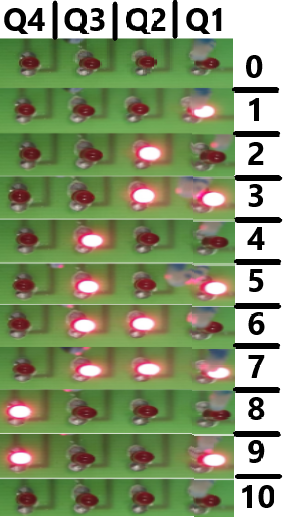
\includegraphics[width=0.95\textwidth,height=13cm]{./figures/messungen/4bit/wahrheit.png}
  \caption{Diese Abbildung beinhaltet die gemessenen logischen Ausgangszustände
    der $QN$ Ausgänge bei einer Serie an Eingangspulsen. Dabei sind $QN$ die
    $(N-1)$ten Bits des gebauten 4Bit dekadischen synchron Zählers. Die Zahlen
    in der rechten Spalte entsprechen dem j-ten gegebenen Puls im
  Eingangssignal \textit{CLK}.Eine leuchtende LED entspricht einem
\textit{HIGH}-, eine nicht leuchtende entspricht einem \textit{LOW}-Signal}
  \label{fig:mess_wahrheitstabelle_alarm}
\end{figure}

% Für die Untersuchung des Master-Switches im ausgeschalteten Zustand wurden die
% zuvor \textit{wahren} Eingangssignalkombinationen durchgeschaltet und überprüft, ob diese
% nicht die Alarmanlage ($y$) anschlagen lassen. Da die Schaltung zuvor, wie in
% \autoref{fig:mess_wahrheitstabelle_alarm} ersichtlich, funktionierte, ist
% dadurch die Funktionstüchtigkeit des Master-Switches gezeigt.

% zu 4: Auswertung siehe EPM Skript nur Besprechung von Umformungen und 
% Sachen die man mit den Messungen machen muss damit man Conclusion und Wissen 
% gewinnen kann.
% Entsprechend der in Punkt 2. angegebenen Beziehungen (Formeln) ist aus den
% Messergebnissen in Punkt 5. das in Punkt 1. formulierte Endergebnis zu
% berechnen. Oft ist eine Ermittlung des Endergebnisses aus einer grafischen
% Darstellung bzw. eine grafische Veranschaulichung zweckmaßig. Dabei kann
% die Verwendung von Millimeterpapier oder Computerprogrammen hilfreich sein.
% Wenn eine Bearbeitung der Daten auf dem Computer erfolgt, sollte bei der
% Darstellung der Graphen eine sinnvolle Skalenteilung des Koordinatensystems
% gemacht werden. Die Unsicherheitsbetrachtung f ̈ur die angegebenen Messwerte,
% sowie fur Zwischen- und Endergebnisse ist in diesem Abschnitt
% nachvollziehbar zu beschreiben. Dabei ist nach Kapitel 1 vorzugehen und
% insbesondere auf die Klassifizierung der Unsicherheit (Typ-A/B) und die
% Unsicherheitsfortpflanzung einzugehen.
\section{Auswertung}\label{sec:Auswertung}
In diesem Protokoll ist keine Auswertung von Nöten, da die geforderten Resultate
direkt aus den Ergebnissen der Laborübung folgen. Dennoch wurde für bessere 
Nachvollziehbarkeit die Daten aus \autoref{fig:sim_alarm_wahrheit} nochmals mit Farben
hinterlegt und die \textit{HIGH} Zustände mit einer 1 markiert. 

\begin{figure}[H]
  \centering
    % 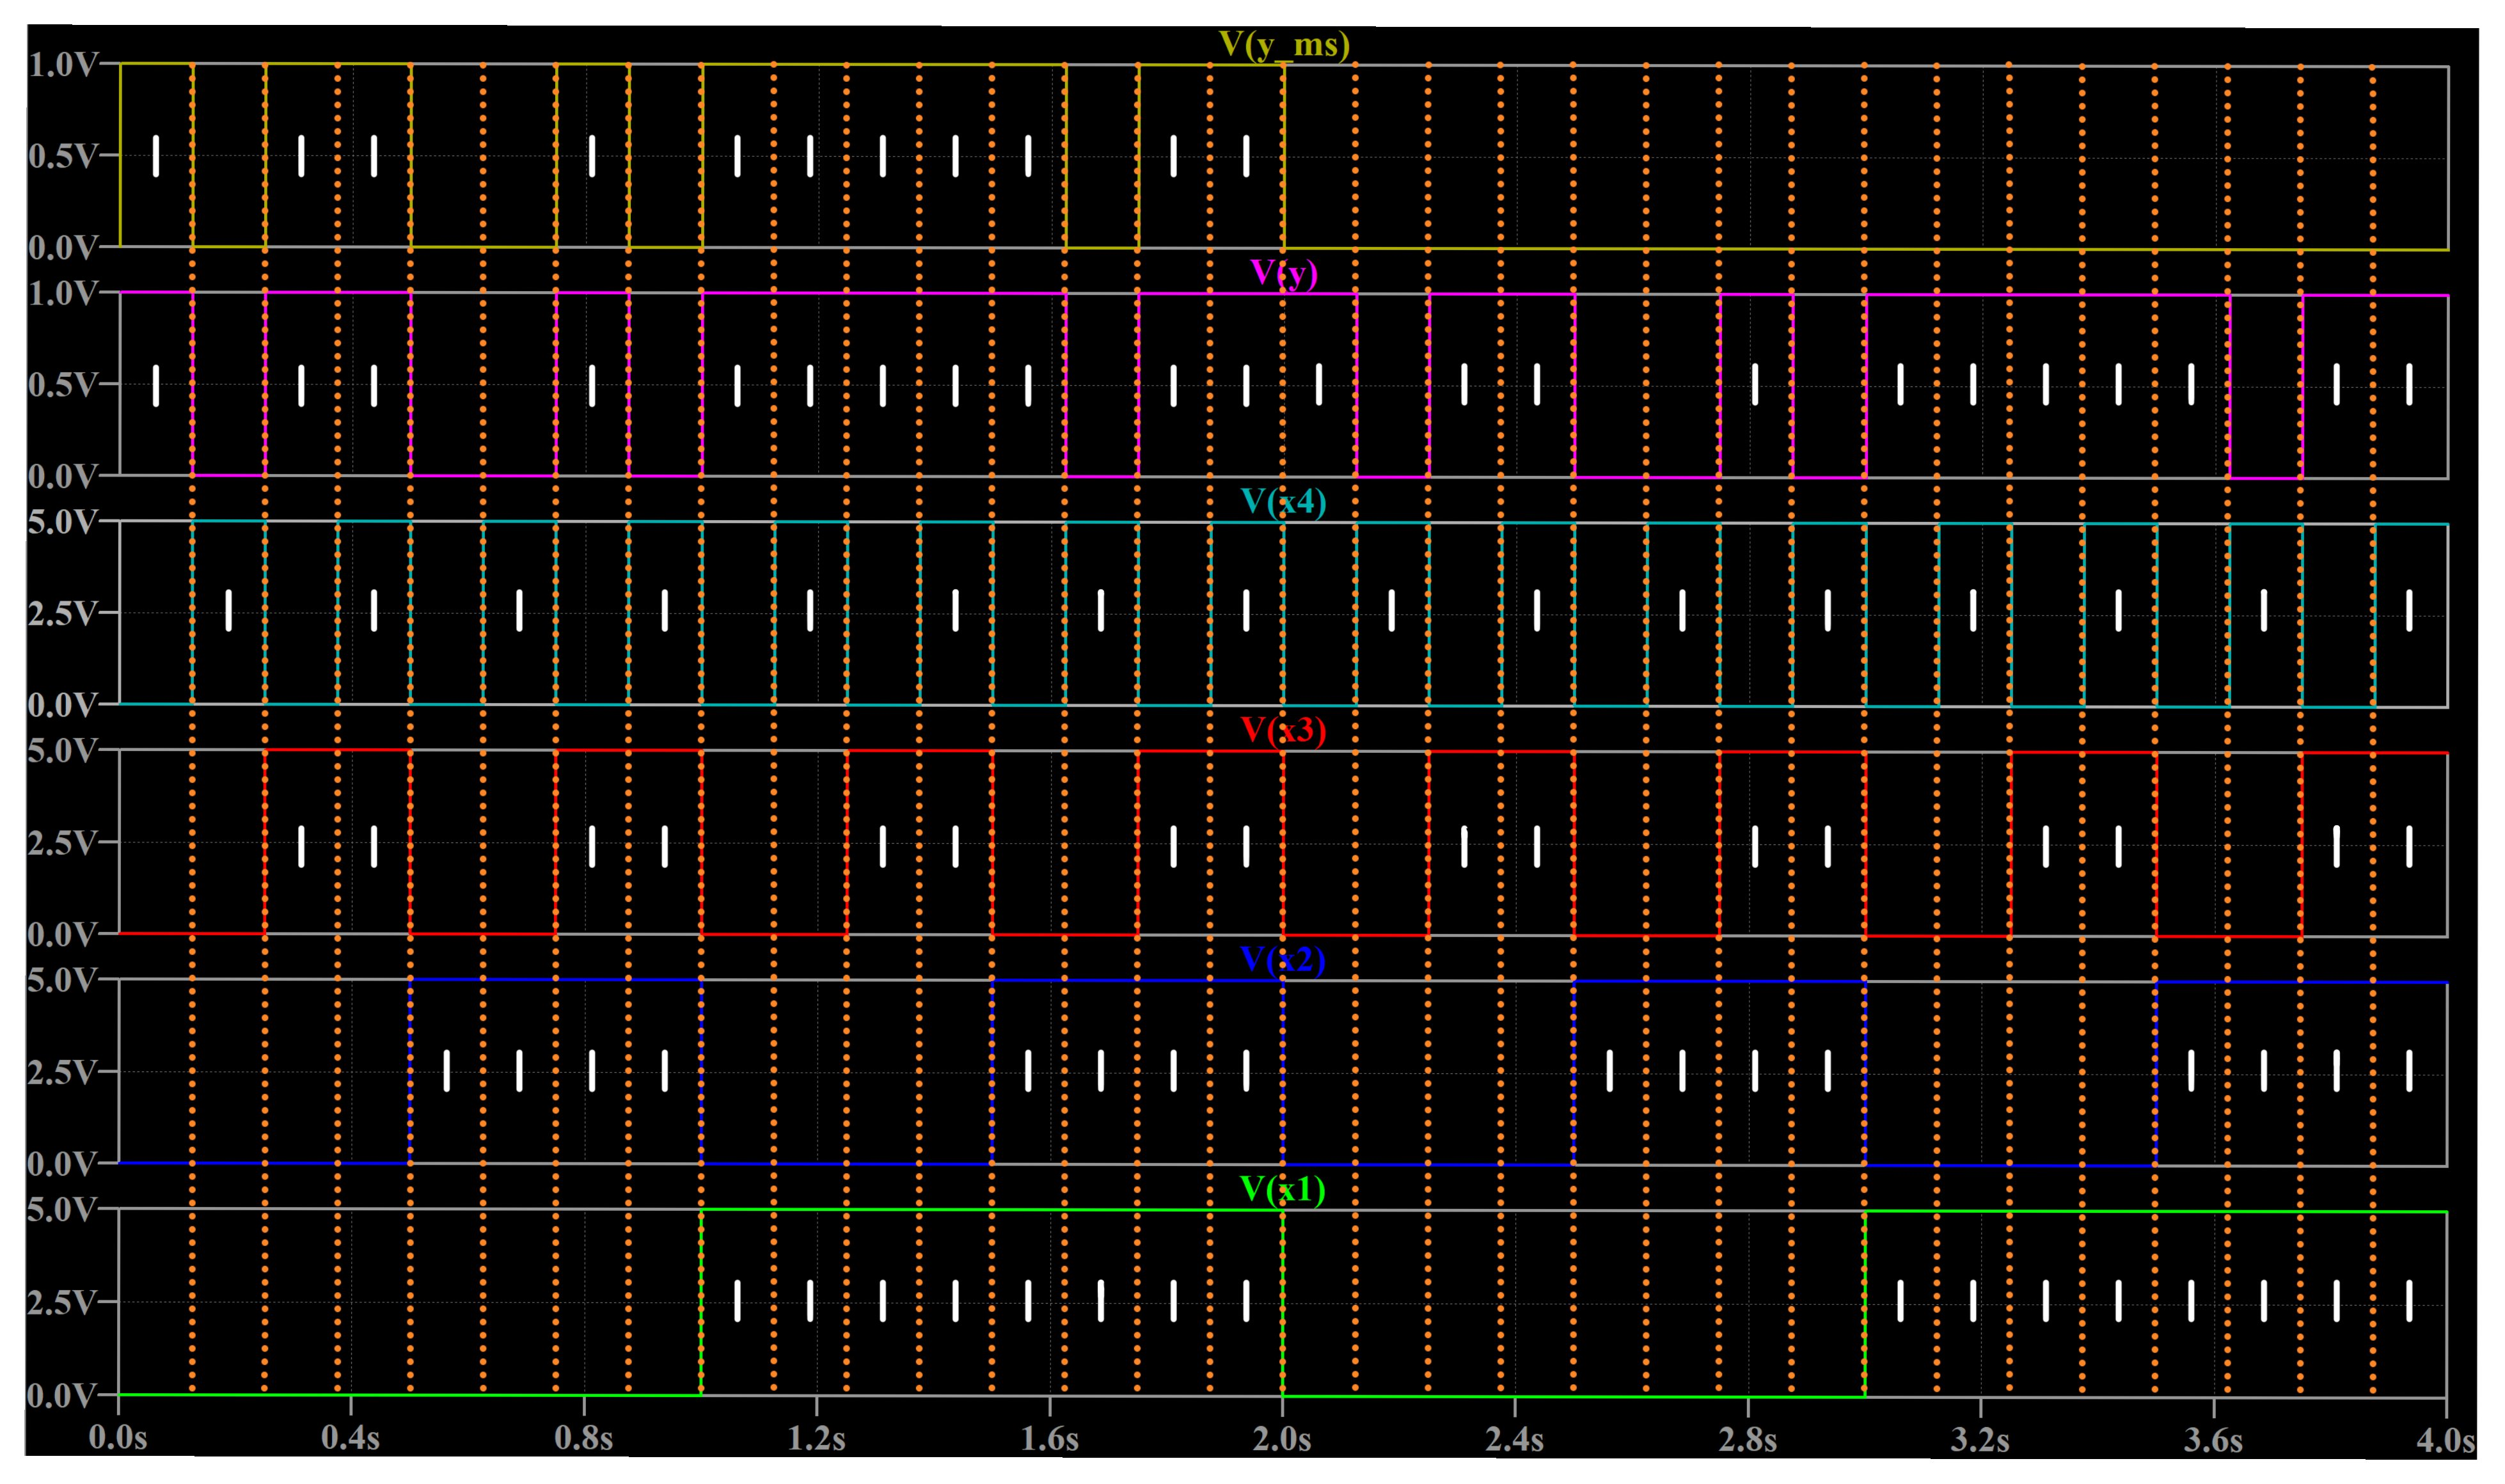
\includegraphics[width=0.95\textwidth]{./simdaten_lab/logic/auswertungalarm.jpg}
  \caption{Diese Grafik spiegelt das Verhalten der
    Einbruchssicherungsschaltung (aus \autoref{fig:sim_aufbau_4bit}) wider, indem alle
    möglichen Eingangssignale durchgeschaltet worden sind und die Response an den
    Ausgängen aufgezeichnet wurde (entsprechend Wahrheitstafel).Dabei sind $x1$, $x2$, $x3$, $x4$ \&
    der \textit{Master-Switch} die Eingangssignale und $y$ das Ausgangssignal sowie $y_ms$
    das Ausgangssignal mit \textit{Master-Switch}. Die
    SPICE-Directive der Simulation ist \texttt{.tran 0 4 0}; die
    Einstellungen der Eingangssignale können der \autoref{fig:sim_aufbau_4bit}
  entnommen werden. Zudem wurden hier die Ticks von einander mittels orange gepunkteten Linien getrennt und die \textit{HIGH} mit 1er markiert.}
  \label{fig:sim_alarm_wahrheit_aus}
\end{figure}

% zu 5: Diskussion und Zusammenfassung
% In der Zusammenfassung stehen noch einmal die wichtigsten Messergebnisse, wobei auf Tabellen und
% Abbildungen nur verwiesen werden soll. Die Ergebnisse sind auch zu diskutieren. Insbesondere müssen
% Abweichungen zwischen Simulation und praktischer Durchführung diskutiert werden.
\section{Diskussion und Zusammenfassung}\label{sec:Diskussion} 
\subsection{Diskussion}
In \autoref{fig:sim_jk_wahrheit} von der Simulation und
\autoref{fig:mess_wahrheitstabelle_jk}, welche die LEDs vom Steckbrett zeigt,
ist das Verhalten eines CMOS-Inverters gut zu erkennen; dabei wird das Signal
am Ausgang relativ zu jenem am Eingang negiert.
Weiters ist anhand von \autoref{fig:sim_jk_wahrheit} aus der Simulation ersichtlich, dass
der Schaltvorgang in CMOS endlich schnell erfolgt. Dabei ist ein deutliches
Maximum des Stroms von \SI{4,21}{\milli \ampere} zu erkennen (siehe \autoref{fig:sim_inv_eingangsstrom}), 
wenn (im Falle des Inverters) beide MOSFETs
leitfähig sind, nämlich am Schnittpunkt der Spannungsverläufe.
Die Spannung an diesen Schnittpunkten beträgt \SI{1,63}{\volt} 
(siehe \autoref{fig:sim_inv_threshold}) und liegt
somit innerhalb der für die Gate-Source-Spannung toleranten Intervalle
von \SIrange{0.8}{2.4}{\volt} beim \textit{ZVN2106A} und von
\SIrange{-3.5}{-1.5}{\volt} beim \textit{ZVP2106A} nach den zugehörigen Datenblättern.

Das aus MOSFETs konstruierte NAND liefert als Ergebnis aller möglichen
Kombinationen der beiden Eingangssignale \autoref{fig:sim_nand_wahrheit} für die Simulation
und \autoref{fig:mess_wahrheitstabelle_nand} für die Steckbrettschaltung.
Somit folgt der Verhalt jenem, der in der Wahrheitstabelle in \autoref{sec:Vorbereitung}
(Vorbereitung) notiert wurde - der Ausgang ist stets \texttt{HIGH}, außer wenn
beide Eingänge auf \texttt{High} sind.

Genauso folgen für die Einbruchsicherungsschaltung \autoref{fig:sim_alarm_wahrheit} 
und \autoref{fig:mess_wahrheitstabelle_alarm}
der konstruierten Wahrheitstabelle in \autoref{sec:Vorbereitung} (Vorbereitung).
Demnach löst der Alarm aus, sofern der \textit{Master-Switch} eingeschaltet ist, 
wenn mindestens
zwei Eingangsvariablen auf \texttt{HIGH} sind.


%Es wäre wohl vernünftiger gewesen, die Schaltung an der Steckplatine zunächst aufzubauen, um etwaige 
%Ungenauigkeiten durch die Widerstände 
\subsection{Zusammenfassung}
Im Rahmen dieser Laborübung wurde das Verhalten von einem CMOS-Inverter (siehe \autoref{fig:sim_jk_wahrheit}
respektive \autoref{fig:mess_wahrheitstabelle_jk}), 
einem aus CMOS konstruierten NAND (siehe \autoref{fig:sim_nand_wahrheit}
respektive \autoref{fig:mess_wahrheitstabelle_nand}) und einer Einbruchsicherungsschaltung 
(=Schaltnetz mit 4 Eingangsvariablen
und \textit{Master-Switch}; siehe \autoref{fig:sim_alarm_wahrheit_aus}
respektive \autoref{fig:mess_wahrheitstabelle_alarm}) erfolgreich mittels 
Simulation und mithilfe von LEDs an Steckbrettschaltungen
verifiziert.
\newpage

\printbibliography

\listoffigures

\listoftables



\end{document}


